%%
%% Template appendix.tex
%%

\appendix

\chapter{How to Obtain the Datasets}
\label{cha:datasets}

To get all 800 million objects:

\begin{minted}[fontsize=\footnotesize, frame=single, tabsize=4]{sql}
SELECT
p.ra, p.dec,
CASE s.class WHEN 'GALAXY' THEN 'Galaxy'
WHEN 'STAR' THEN 'Star'
WHEN 'QSO' THEN 'Quasar'
END AS class,
s.subclass,
s.z AS redshift,
s.zErr AS redshiftErr,
s.zWarning,
p.psfMag_u, p.psfMagErr_u,
p.psfMag_g, p.psfMagErr_g,
p.psfMag_r, p.psfMagErr_r,
p.psfMag_i, p.psfMagErr_i,
p.psfMag_z, p.psfMagErr_z,
p.petroMag_u, p.petroMagErr_u,
p.petroMag_g, p.petroMagErr_g,
p.petroMag_r, p.petroMagErr_r,
p.petroMag_i, p.petroMagErr_i,
p.petroMag_z, p.petroMagErr_z,
p.extinction_u, p.extinction_g, p.extinction_r,
p.extinction_i, p.extinction_z,
p.petroRad_r, p.petroRadErr_r

FROM PhotoObj AS p
LEFT JOIN SpecObj AS s
ON s.bestobjid = p.objid
\end{minted}


Getting the main labelled SDSS dataset:

\begin{minted}[fontsize=\footnotesize, frame=single, tabsize=4]{sql}
SELECT
	-- right ascension and declination in degrees
	p.ra, p.dec,
	
	-- class of object, expert opinion (galaxy, star, or quasar)
	CASE s.class WHEN 'GALAXY' THEN 'Galaxy'
	WHEN 'STAR' THEN 'Star'
	WHEN 'QSO' THEN 'Quasar'
	END AS class,
	
	s.subclass, -- subclass of object
	
	-- redshift of object from spectrum with error, expert opnion
	s.z AS redshift,
	s.zErr AS redshiftErr,
	s.zWarning,
	
	-- PSF magnitude measurements in 5 bands (ugriz) with error
	p.psfMag_u, p.psfMagErr_u,
	p.psfMag_g, p.psfMagErr_g,
	p.psfMag_r, p.psfMagErr_r,
	p.psfMag_i, p.psfMagErr_i,
	p.psfMag_z, p.psfMagErr_z,
	
	-- Petrosian magnitude measurements in 5 bands (ugriz) with error
	p.petroMag_u, p.petroMagErr_u,
	p.petroMag_g, p.petroMagErr_g,
	p.petroMag_r, p.petroMagErr_r,
	p.petroMag_i, p.petroMagErr_i,
	p.petroMag_z, p.petroMagErr_z,
	
	-- extinction values
	p.extinction_u, p.extinction_g, p.extinction_r,
	p.extinction_i, p.extinction_z,
	
	-- size measurement in r-band in arc seconds
	p.petroRad_r, p.petroRadErr_r
	
FROM PhotoObj AS p
JOIN SpecObj AS s
ON s.bestobjid = p.objid

WHERE
	-- only include objects with complete and reasonably accurate data
	p.psfMagErr_u BETWEEN 0 AND 3
	AND p.psfMagErr_g BETWEEN 0 AND 3
	AND p.psfMagErr_r BETWEEN 0 AND 3
	AND p.psfMagErr_i BETWEEN 0 AND 3
	AND p.psfMagErr_z BETWEEN 0 AND 3
	AND p.petroMagErr_u BETWEEN 0 AND 3
	AND p.petroMagErr_g BETWEEN 0 AND 3
	AND p.petroMagErr_r BETWEEN 0 AND 3
	AND p.petroMagErr_i BETWEEN 0 AND 3
	AND p.petroMagErr_z BETWEEN 0 AND 3
	AND p.petroRadErr_r BETWEEN 0 AND 3
	AND s.zErr BETWEEN 0 AND 0.1
	AND s.zWarning = 0    -- spectrum is ok
\end{minted}



\chapter{Guide to Using mclearn}
\label{cha:mclearn}

\section{Installation}
\label{sec:installation}

\section{Usage and Examples}
\label{sec:usage}


\chapter{Vectorisation of the Variance Estimation}
\label{cha:vectorise}

In estimating the variance of the unlabelled pool, there are two matrices we wish to compute...


\chapter{Supplementary Results}

Compare learning curve of multinomial with one-vs-rest in logistic regression.
Compare learning curve of random forest. Warm start


\section{Effects of Dust Extinction on Recall}

\begin{figure}[p]
	\centering
	\begin{subfigure}{\textwidth}
		\centering
		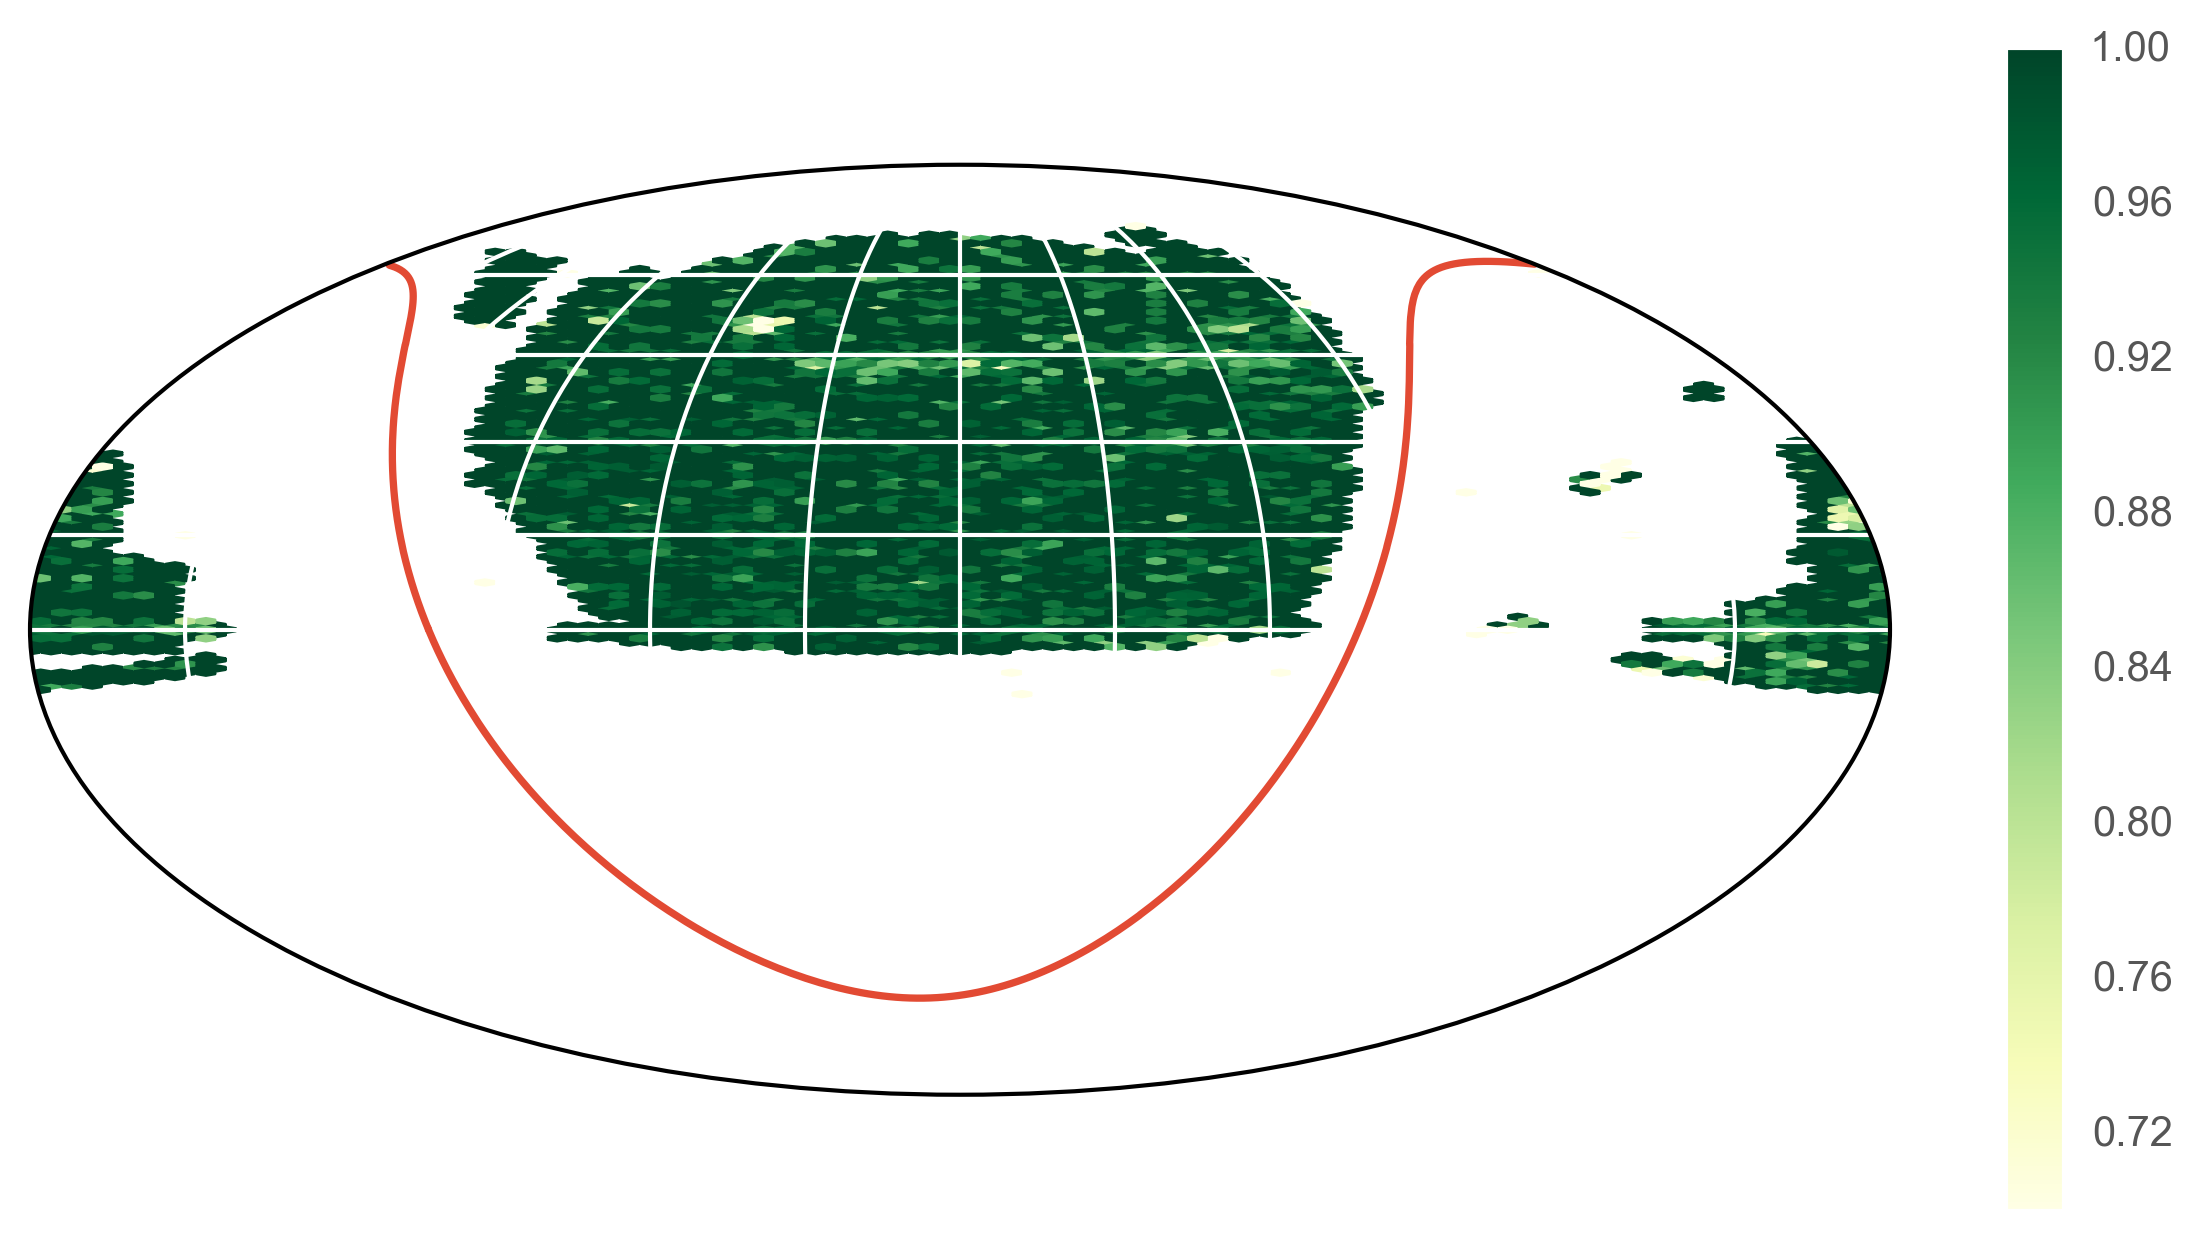
\includegraphics[width=0.75\textwidth]{figures/appendix/map_recall_uncorrected_Galaxy}
		\caption{Recall map of galaxies.}
		\label{fig:map_recall_uncorrected_galaxies}
	\end{subfigure}\\
	\begin{subfigure}{\textwidth}
		\centering
		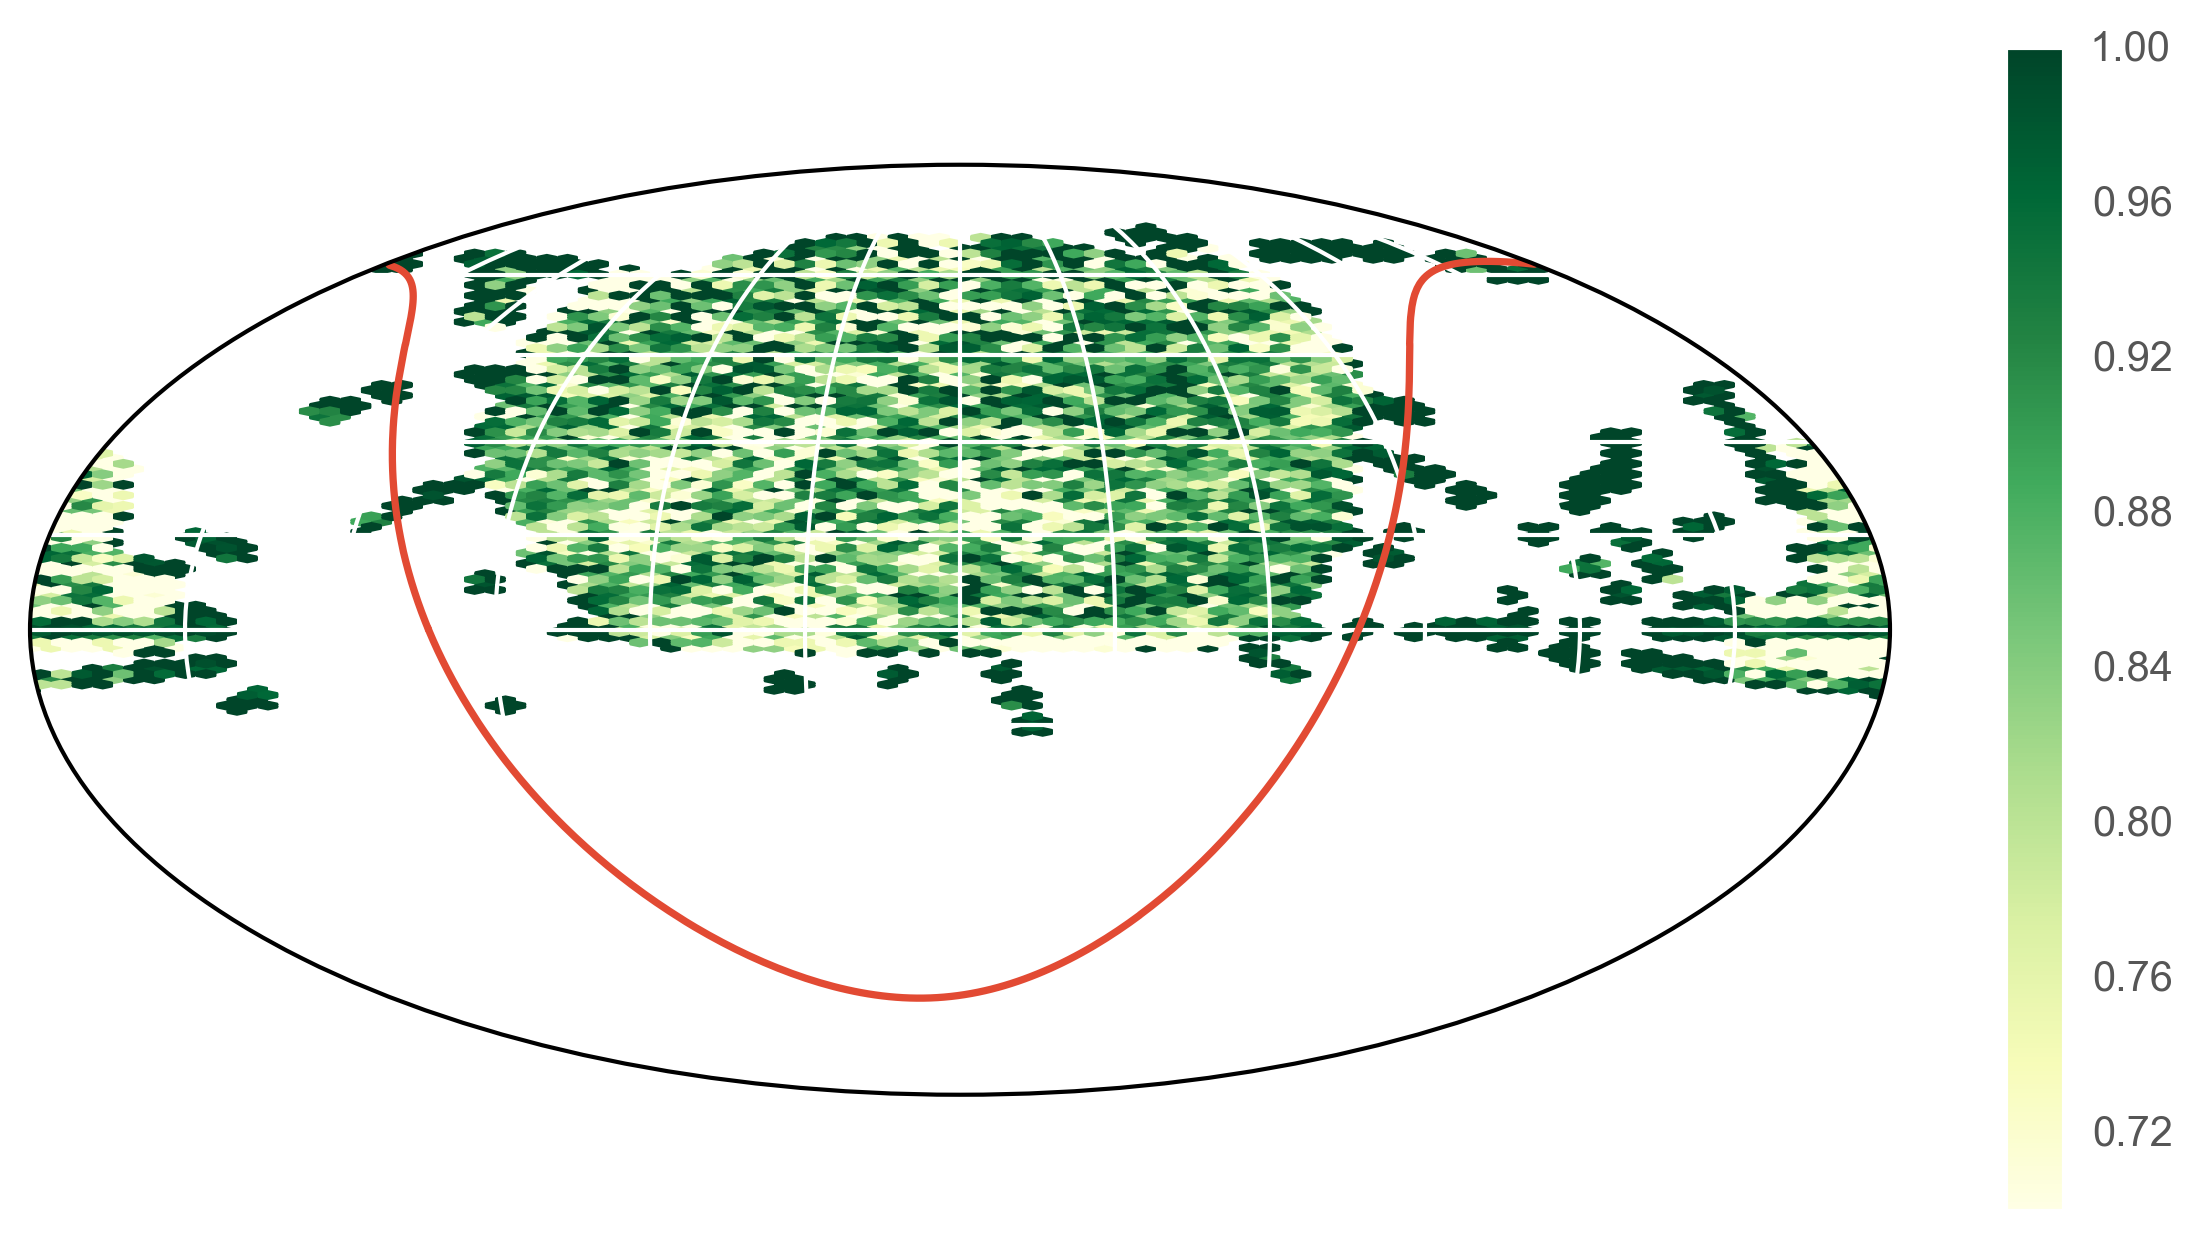
\includegraphics[width=0.75\linewidth]{figures/appendix/map_recall_uncorrected_Star}
		\caption{Recall map of stars.}
		\label{fig:map_recall_uncorrected_stars}
	\end{subfigure}
	\begin{subfigure}{\textwidth}
		\centering
		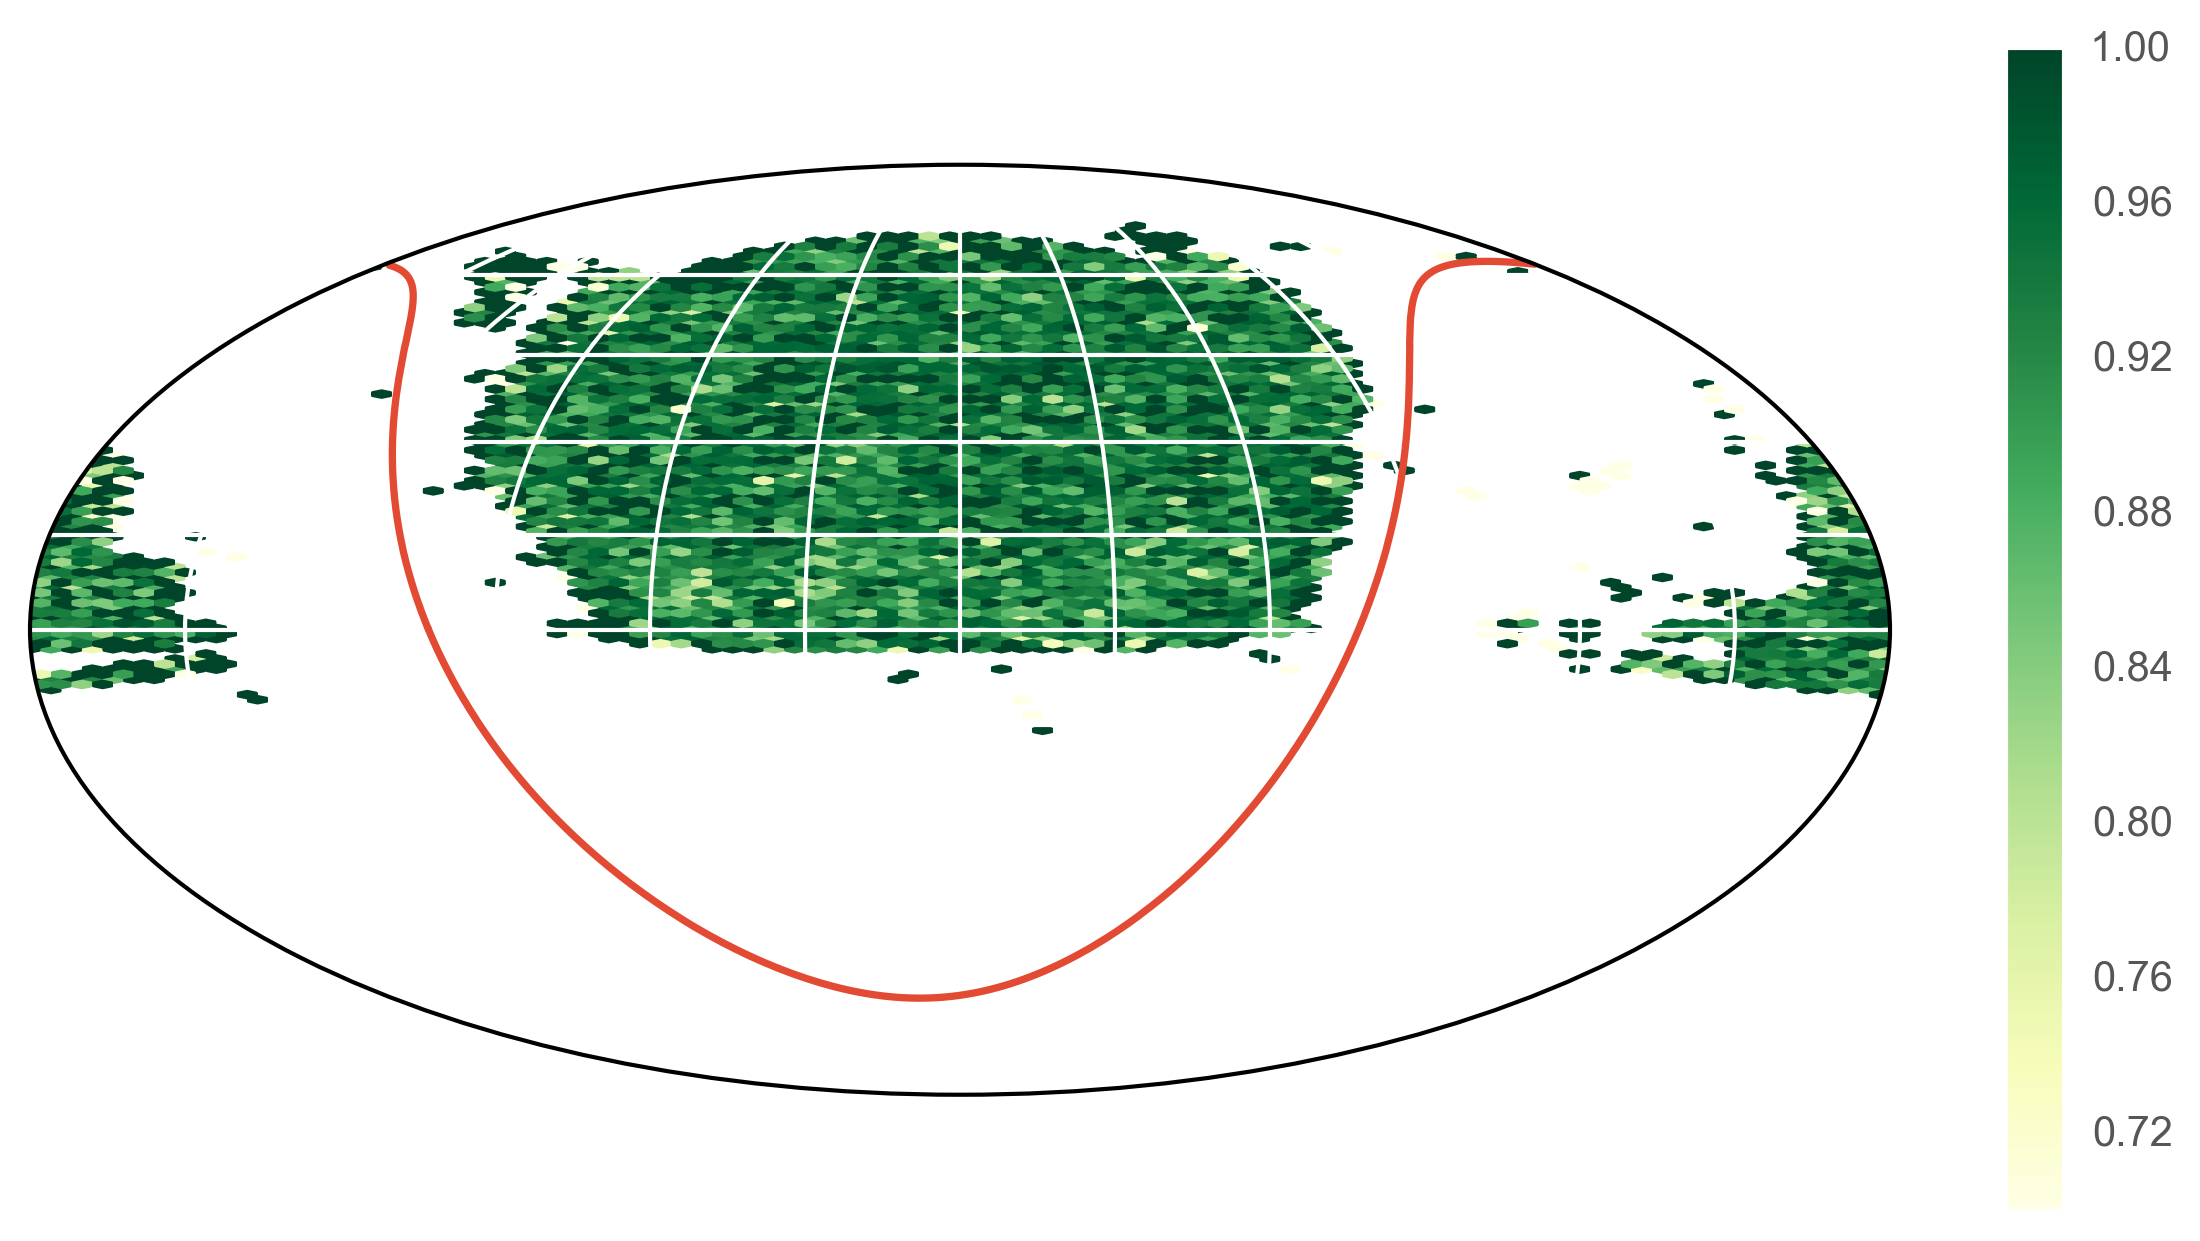
\includegraphics[width=0.75\linewidth]{figures/appendix/map_recall_uncorrected_Quasar}
		\caption{Recall map of quasars.}
		\label{fig:map_recall_uncorrected_quasars}
	\end{subfigure}
	\caption{Recall map of when there is no corrections.}
	\label{fig:map_recall_uncorrected}
\end{figure}


\begin{figure}[p]
	\centering
	\begin{subfigure}{\textwidth}
		\centering
		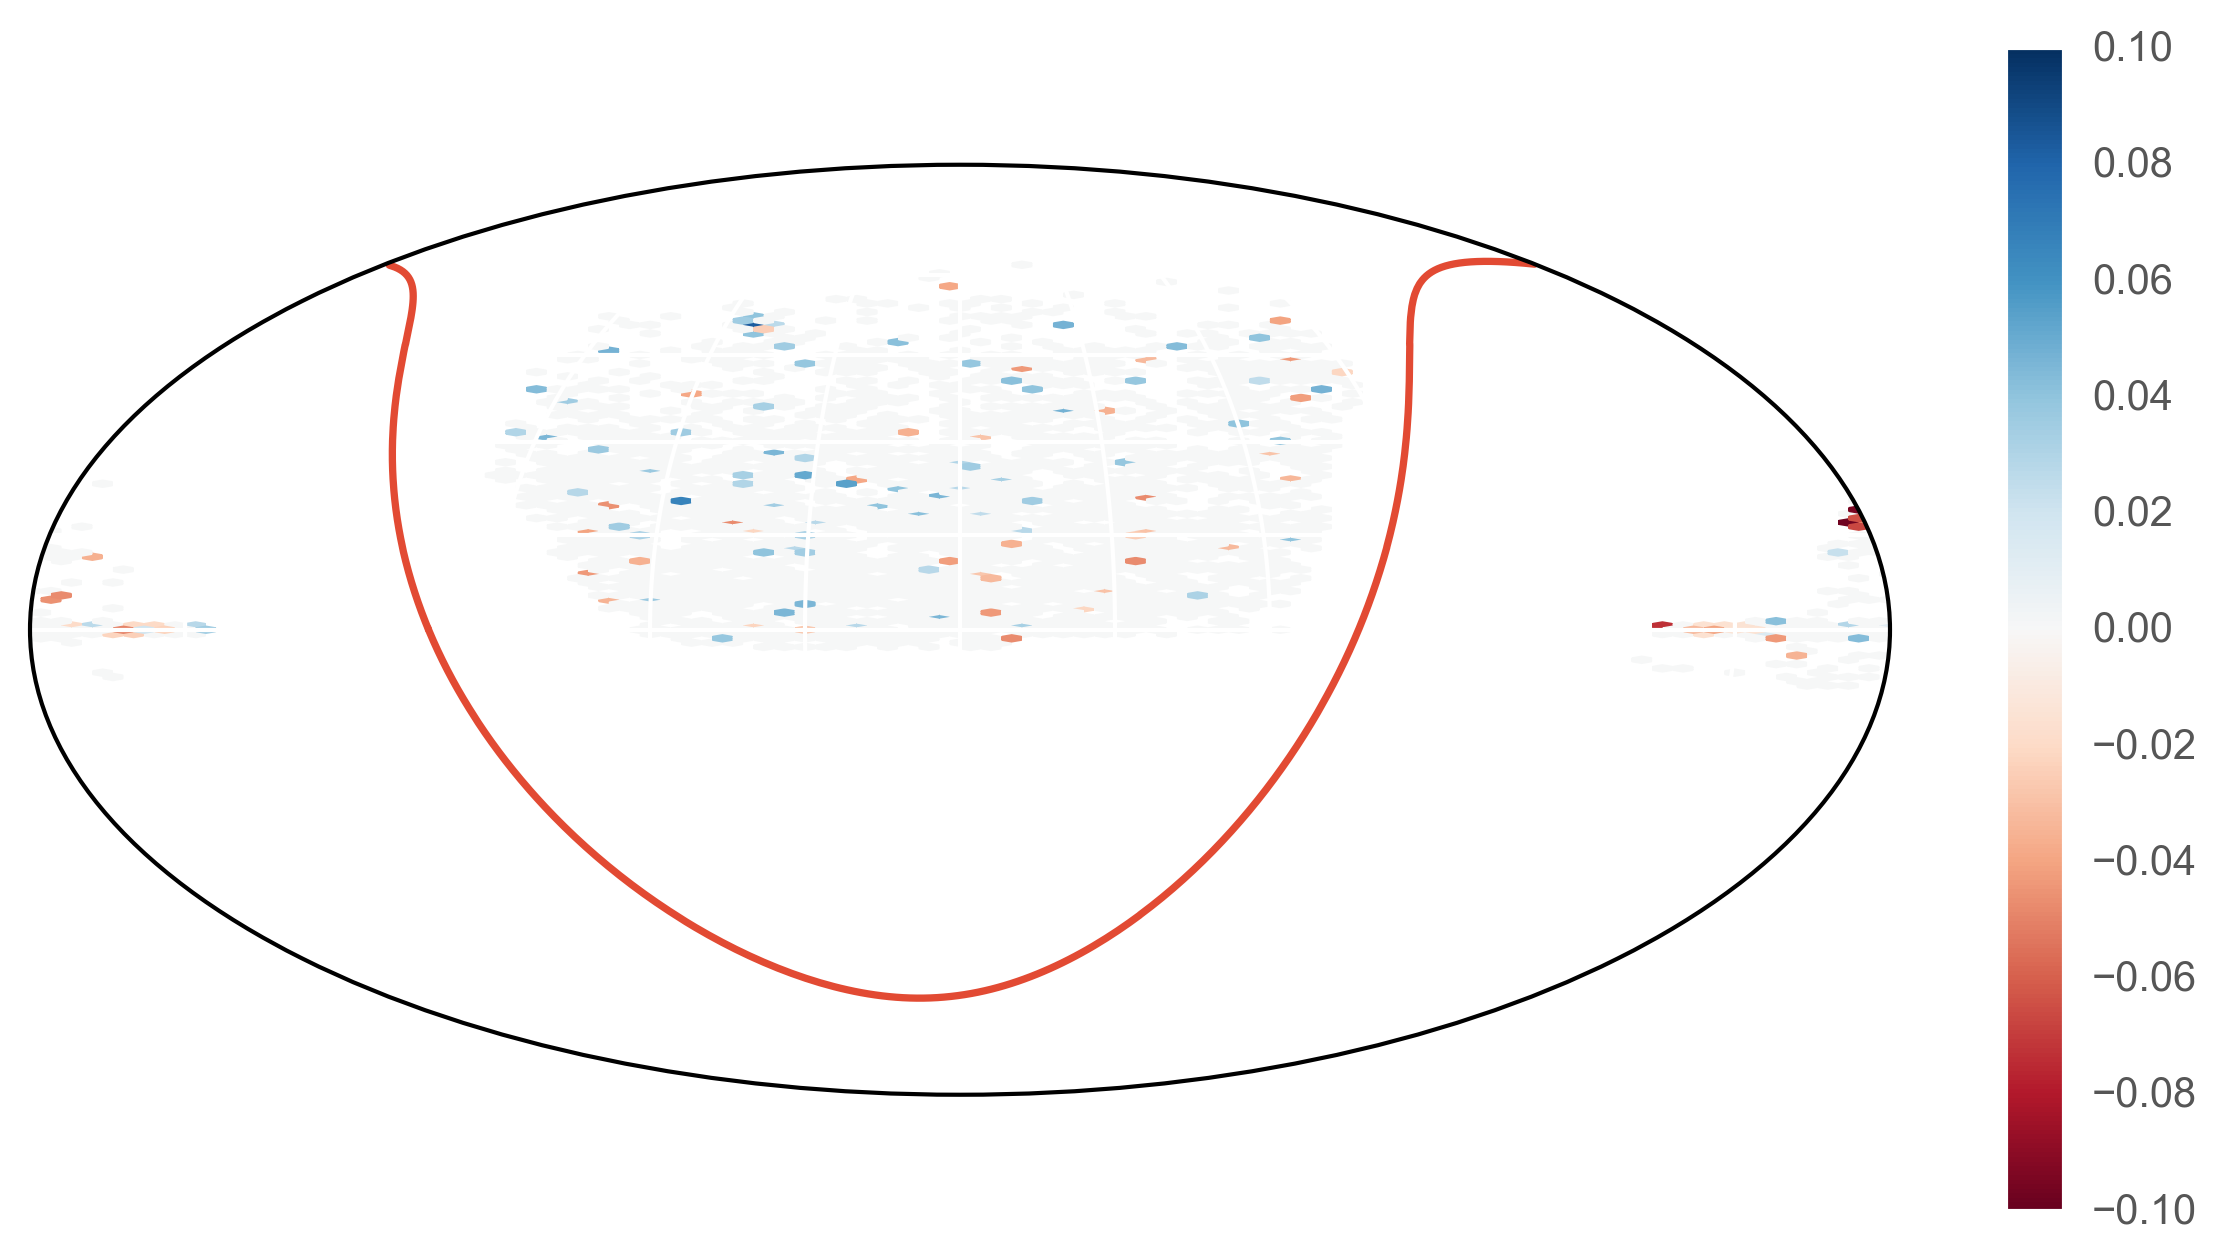
\includegraphics[width=0.75\textwidth]{figures/appendix/map_recall_sfd98_Galaxy}
		\caption{Recall improvement map of galaxies.}
		\label{fig:map_recall_sfd98_galaxies}
	\end{subfigure}\\
	\begin{subfigure}{\textwidth}
		\centering
		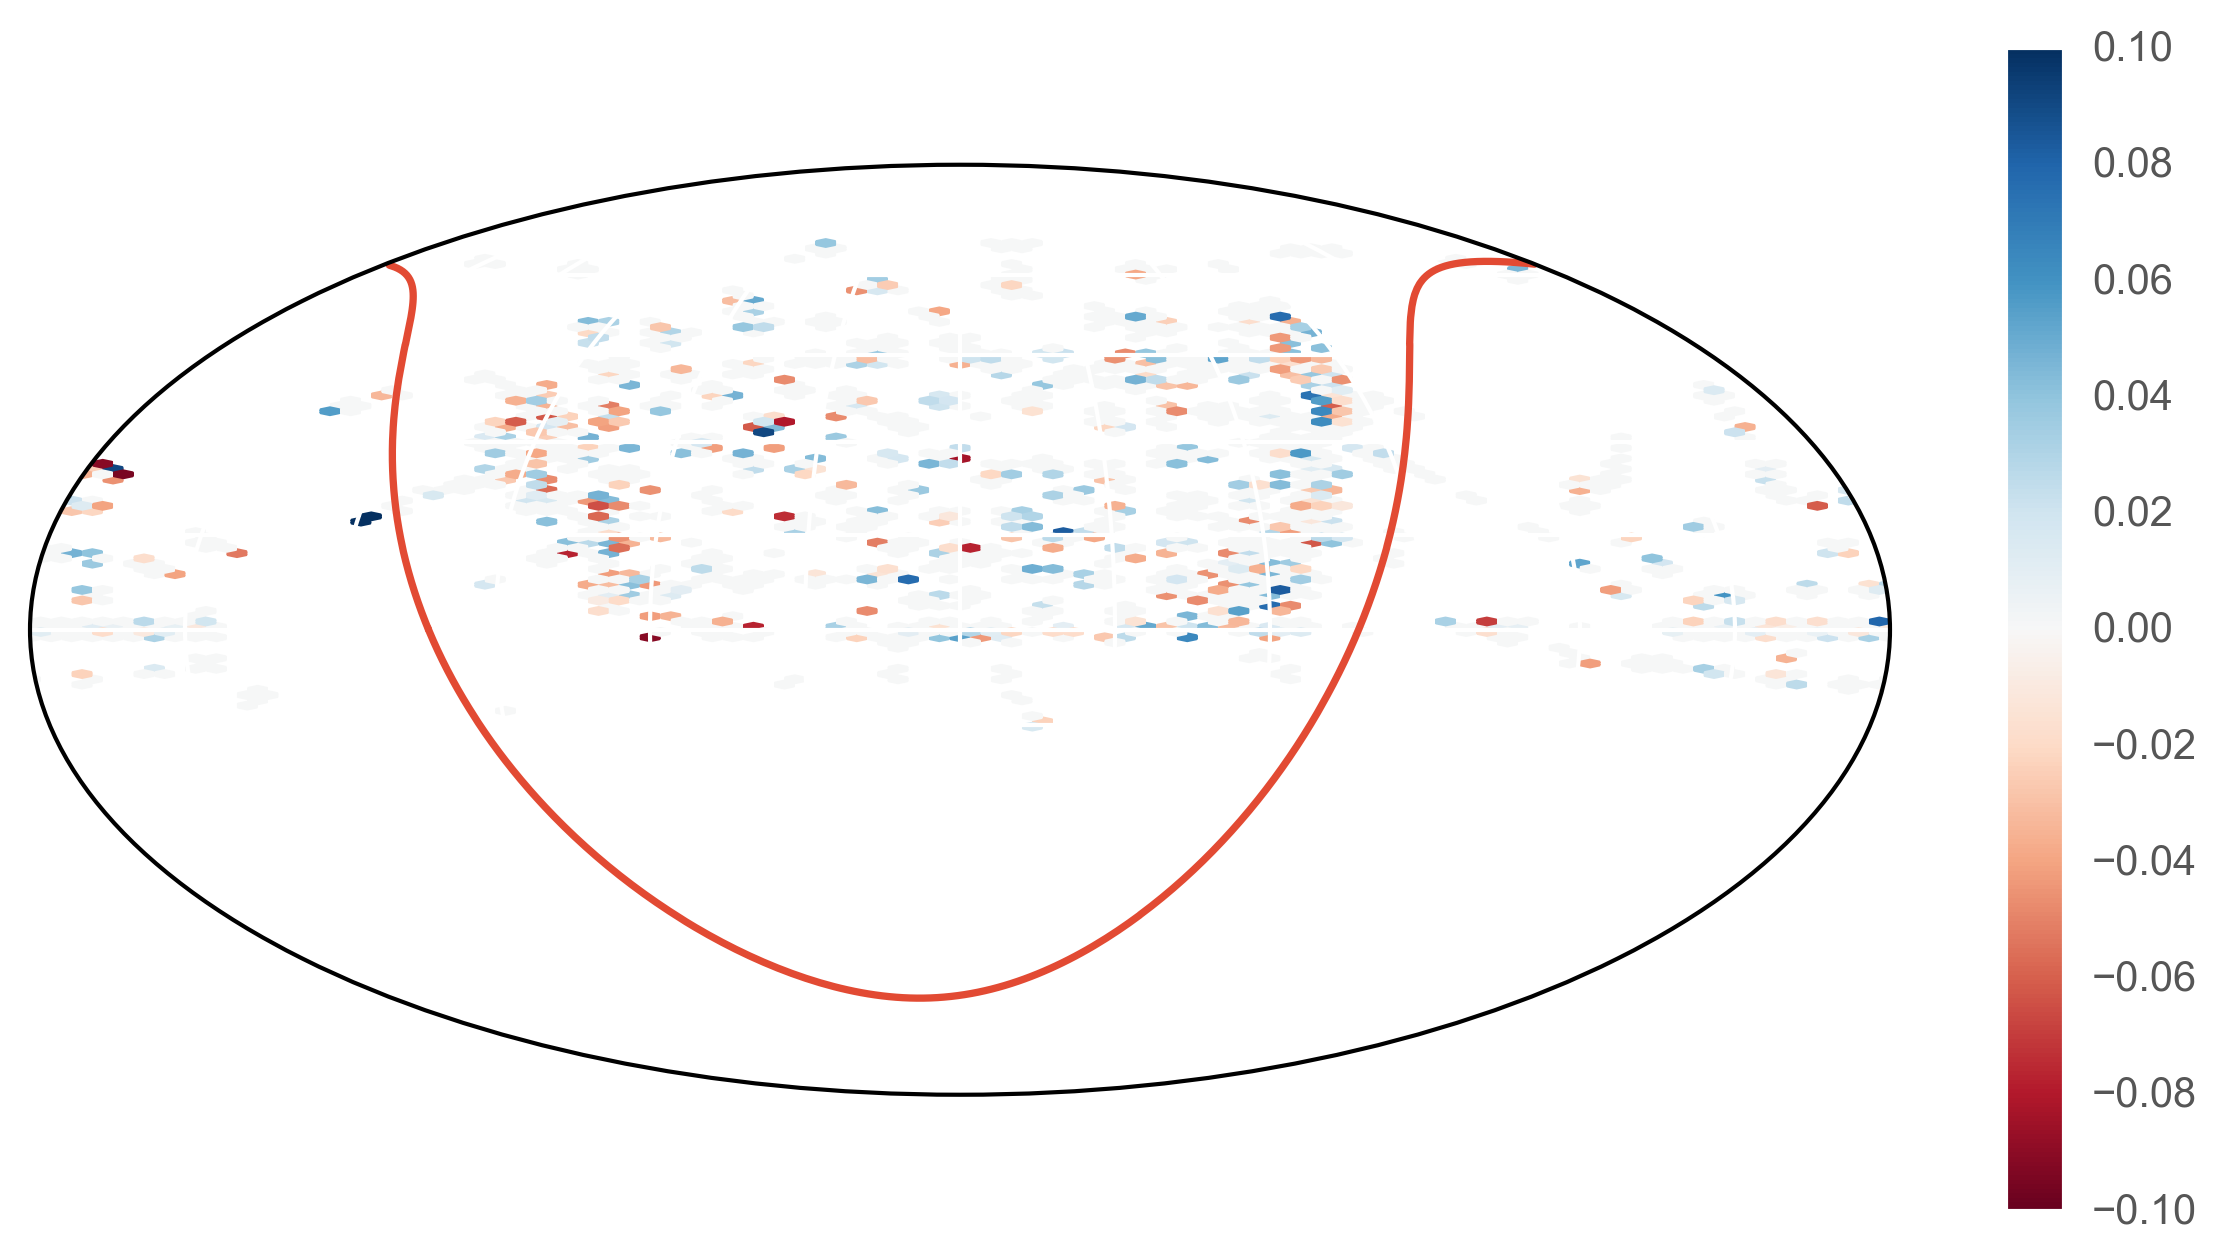
\includegraphics[width=0.75\linewidth]{figures/appendix/map_recall_sfd98_Star}
		\caption{Recall improvement map of stars.}
		\label{fig:map_recall_sfd98_stars}
	\end{subfigure}
	\begin{subfigure}{\textwidth}
		\centering
		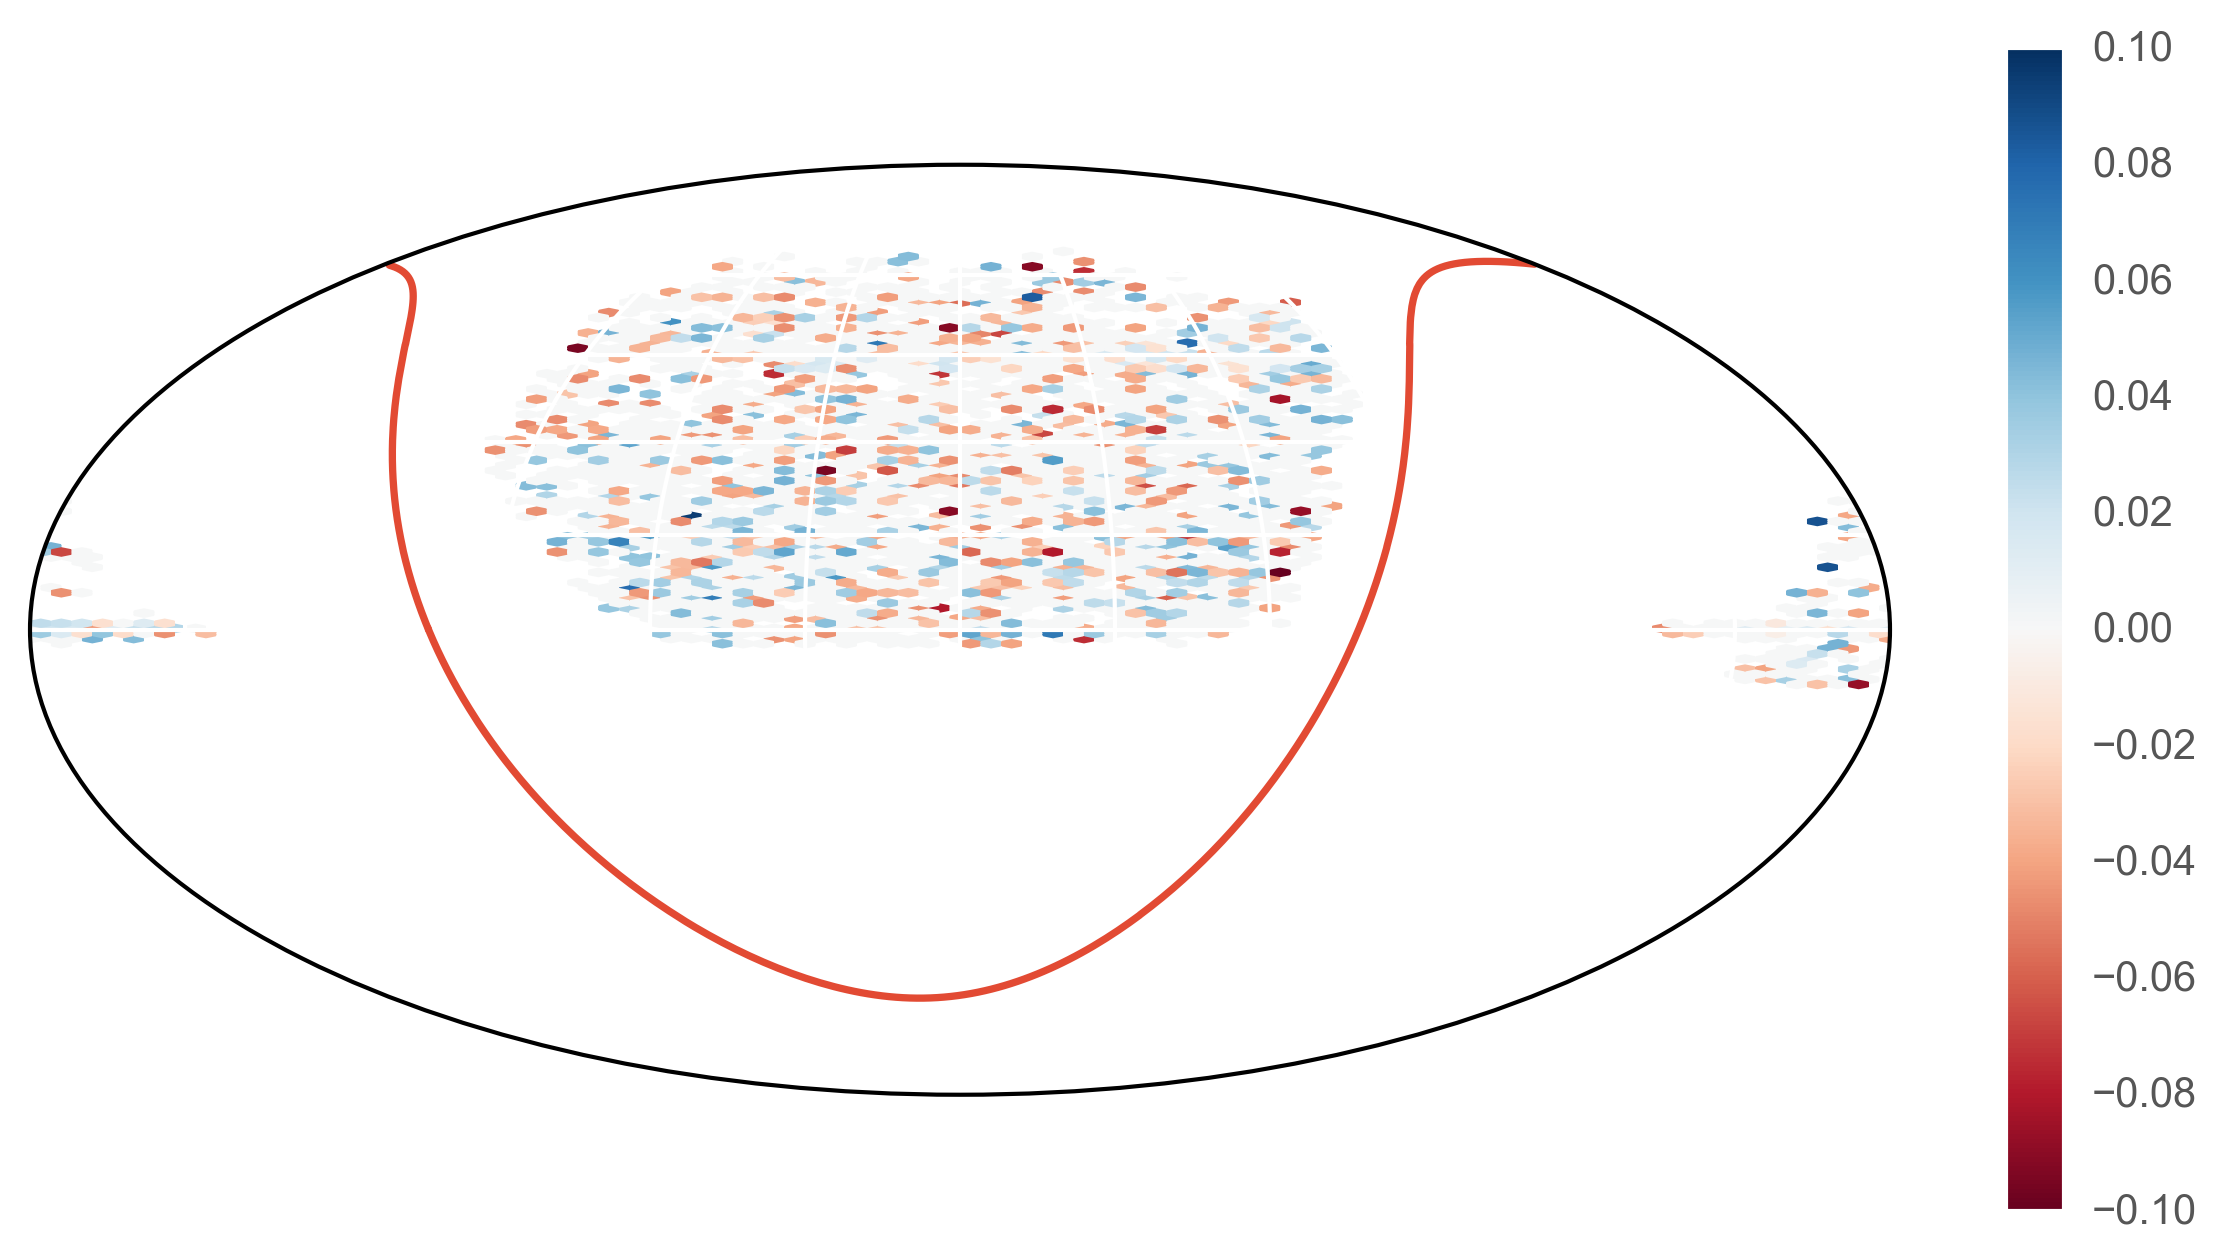
\includegraphics[width=0.75\linewidth]{figures/appendix/map_recall_sfd98_Quasar}
		\caption{Recall improvement map of quasars.}
		\label{fig:map_recall_sfd98_quasars}
	\end{subfigure}
	\caption{Recall improvement map of when the SFD98 correction set is applied.}
	\label{fig:map_recall_sfd98}
\end{figure}


\begin{figure}[p]
	\centering
	\begin{subfigure}{\textwidth}
		\centering
		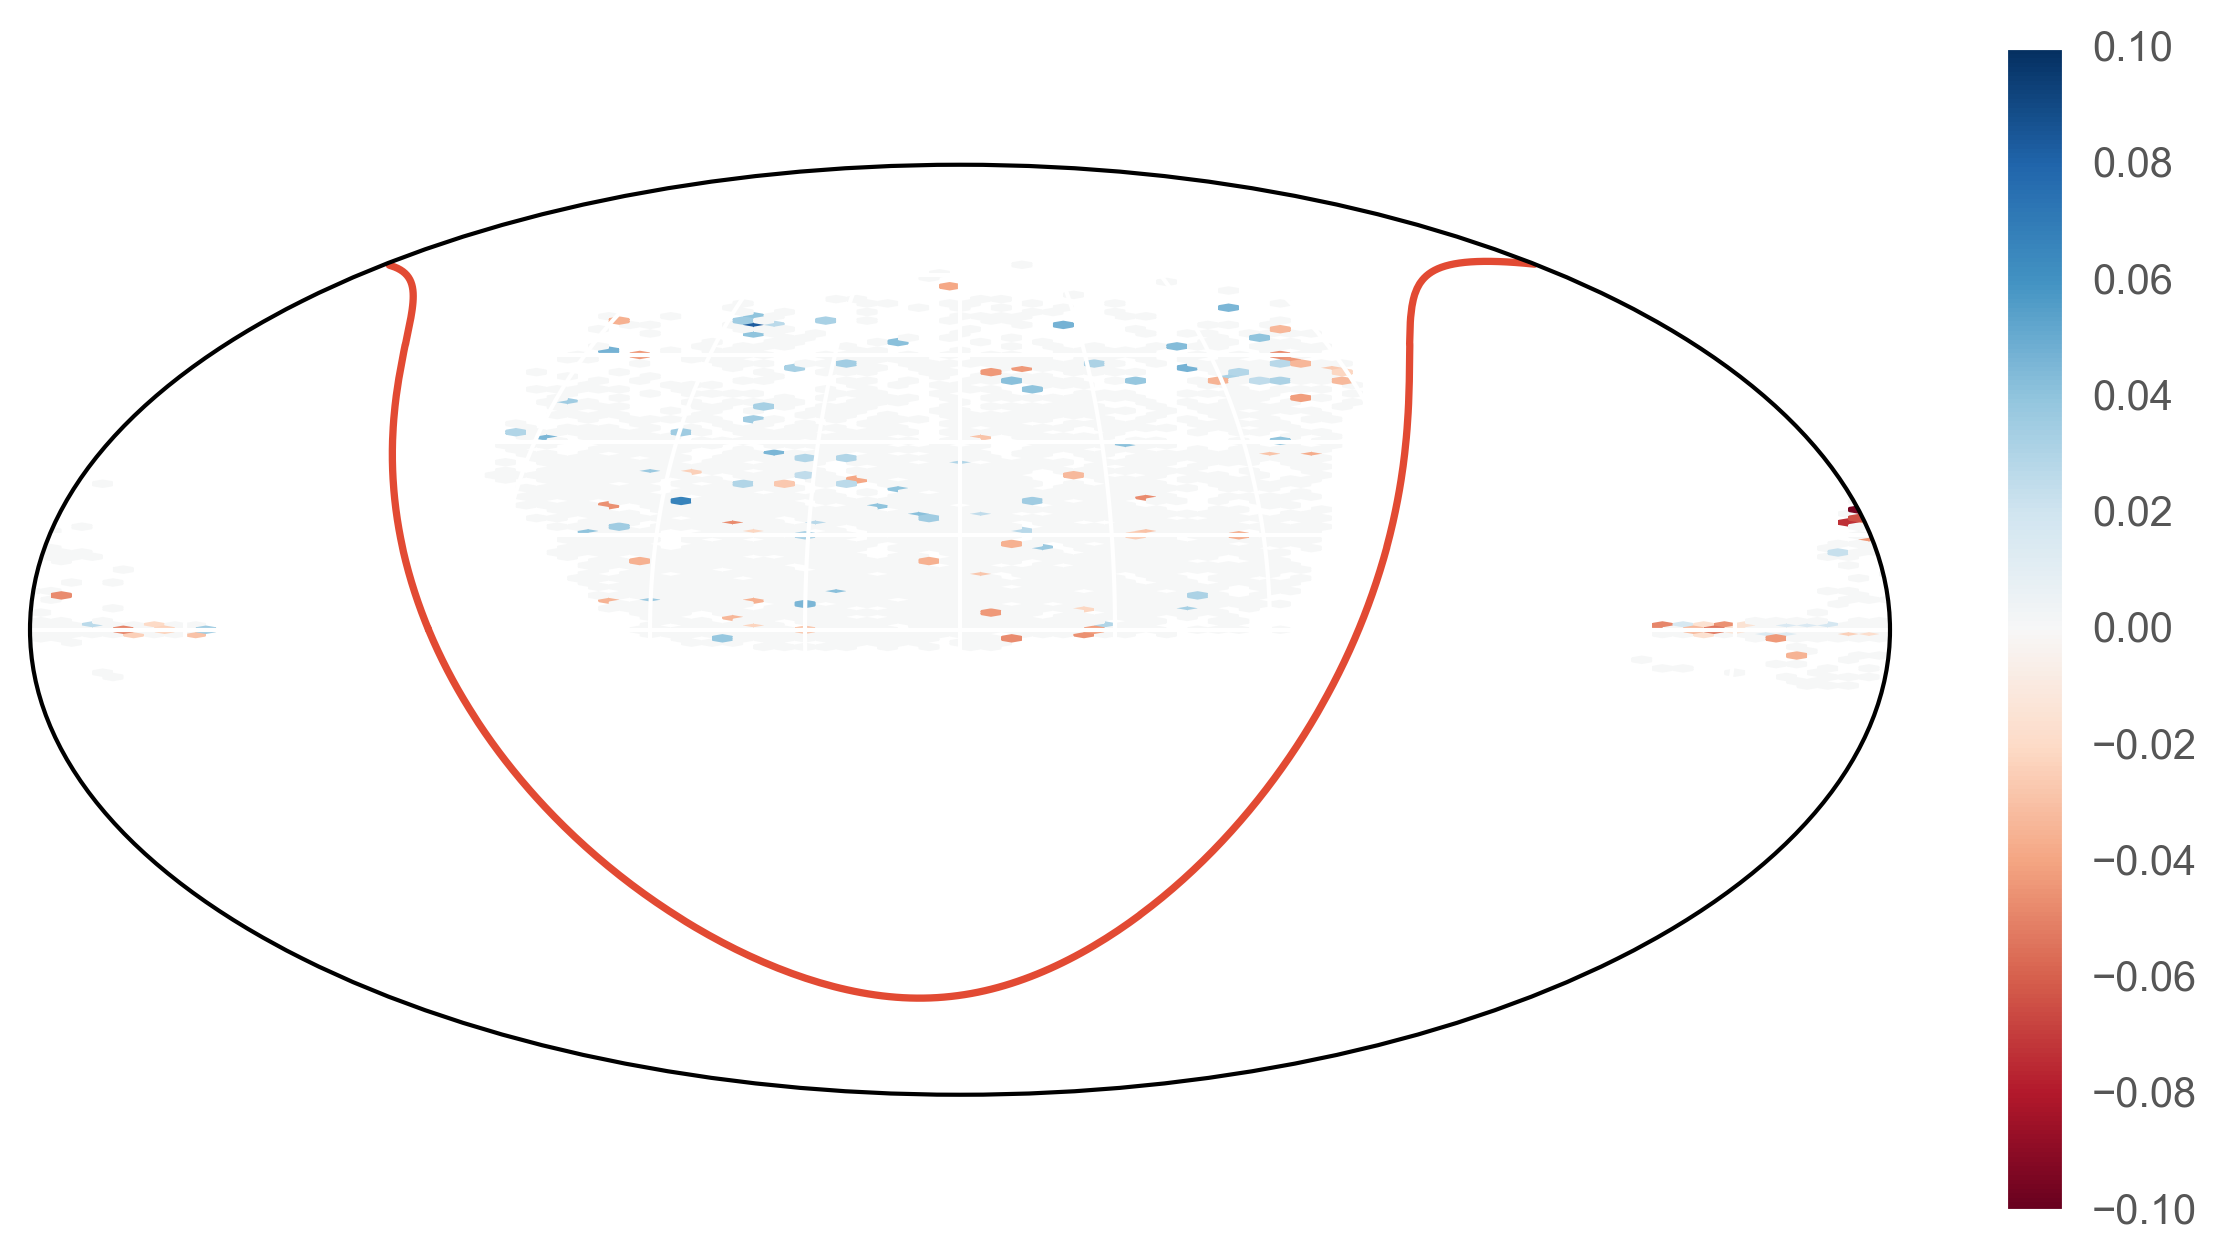
\includegraphics[width=0.75\textwidth]{figures/appendix/map_recall_sf11_Galaxy}
		\caption{Recall improvement map of galaxies.}
		\label{fig:map_recall_sf11_galaxies}
	\end{subfigure}\\
	\begin{subfigure}{\textwidth}
		\centering
		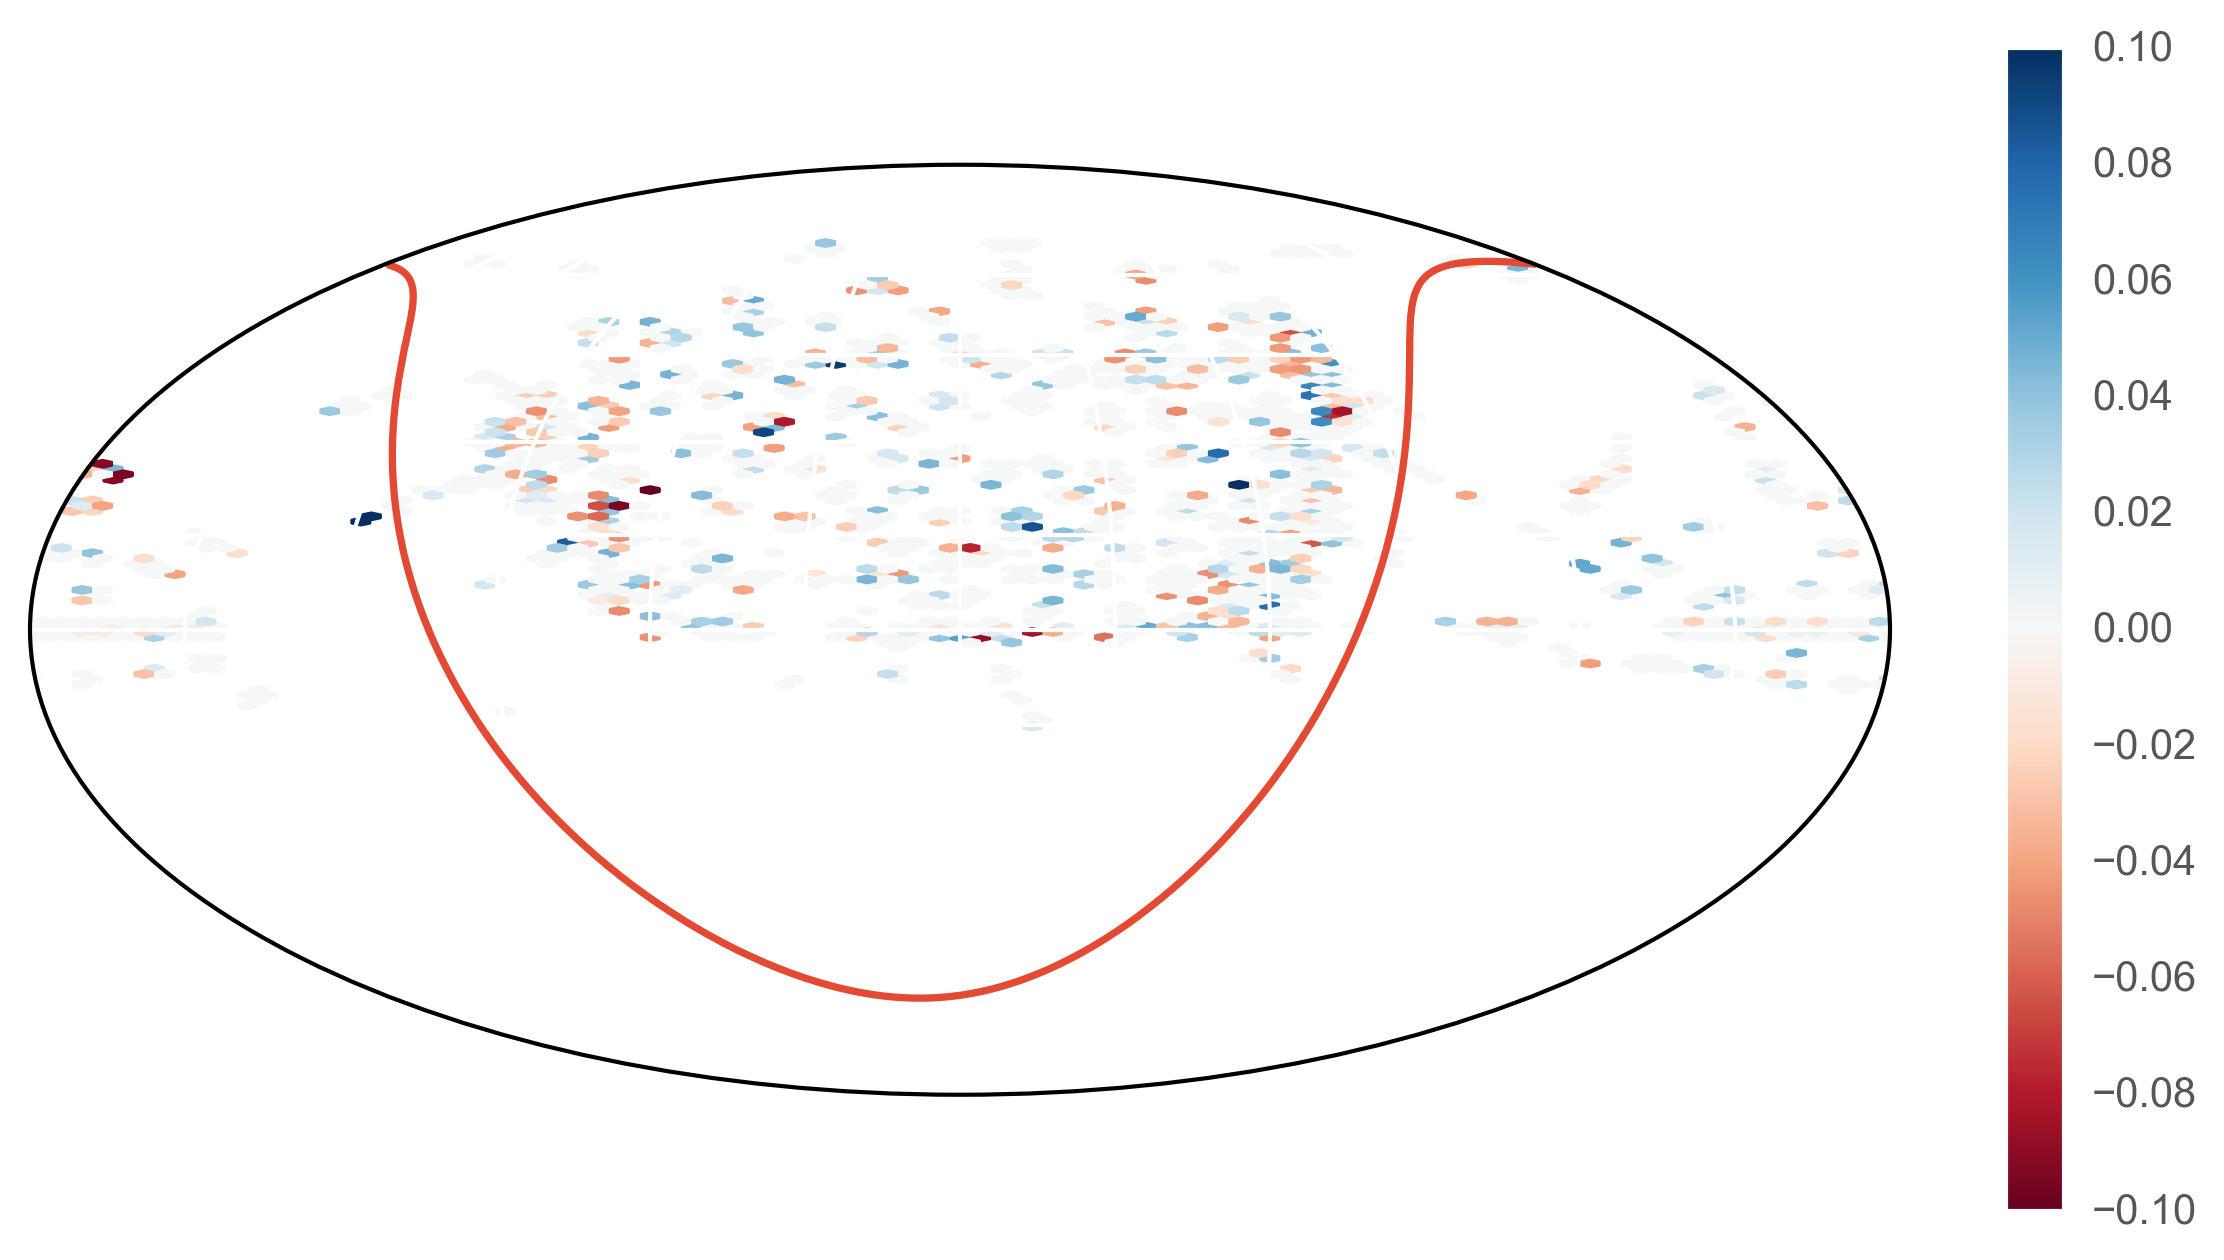
\includegraphics[width=0.75\linewidth]{figures/appendix/map_recall_sf11_Star}
		\caption{Recall improvement map of stars.}
		\label{fig:map_recall_sf11_stars}
	\end{subfigure}
	\begin{subfigure}{\textwidth}
		\centering
		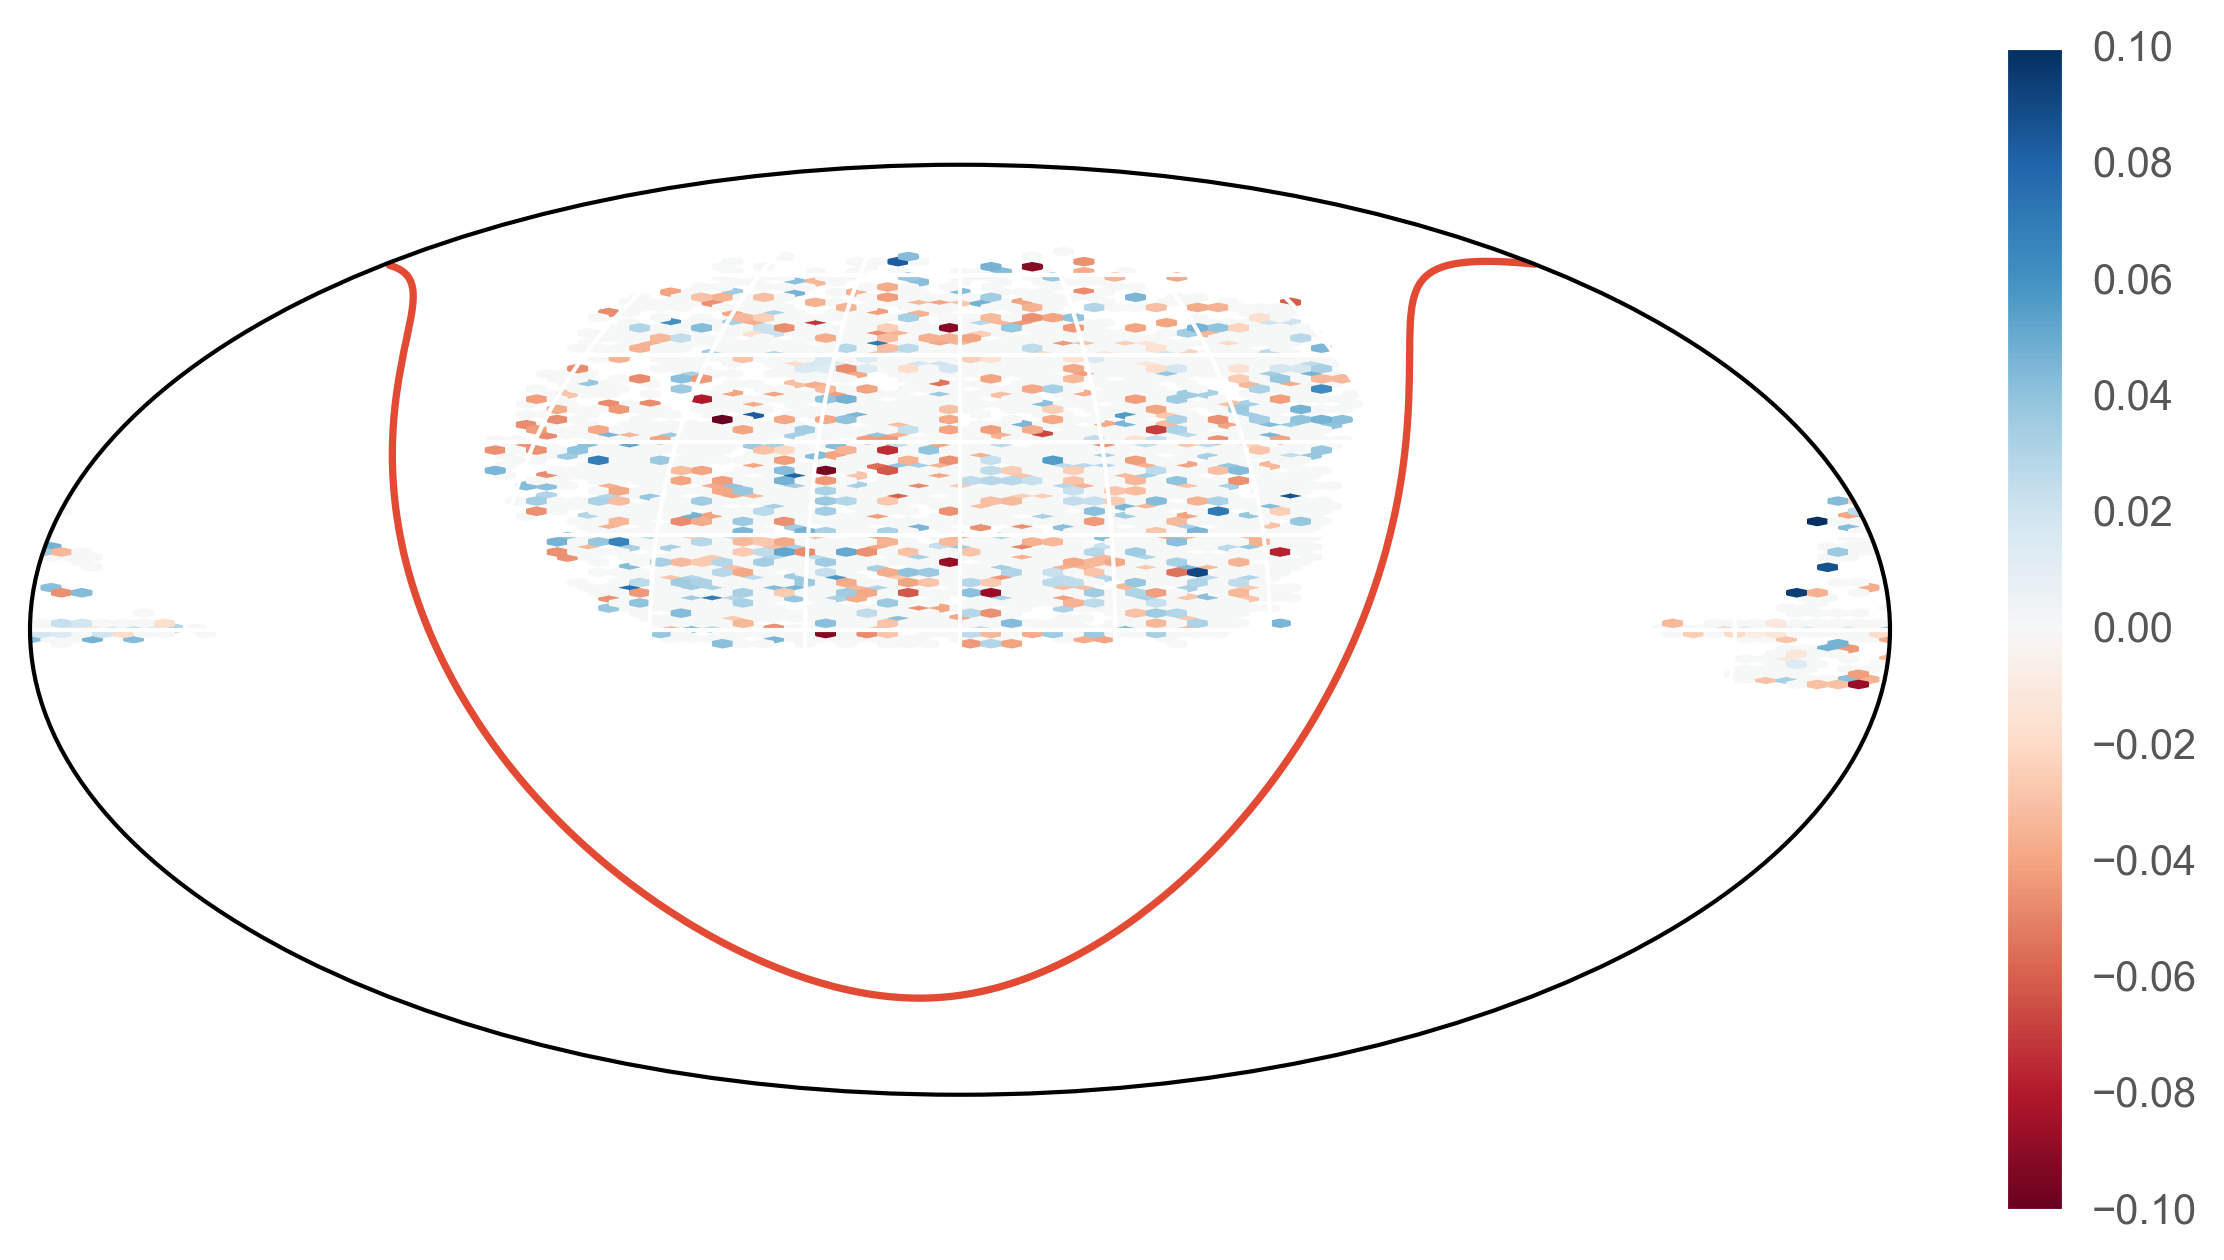
\includegraphics[width=0.75\linewidth]{figures/appendix/map_recall_sf11_Quasar}
		\caption{Recall improvement map of quasars.}
		\label{fig:map_recall_sf11_quasars}
	\end{subfigure}
	\caption{Recall improvement map of when the SF11 correction set is applied.}
	\label{fig:map_recall_sf11}
\end{figure}


\begin{figure}[p]
	\centering
	\begin{subfigure}{\textwidth}
		\centering
		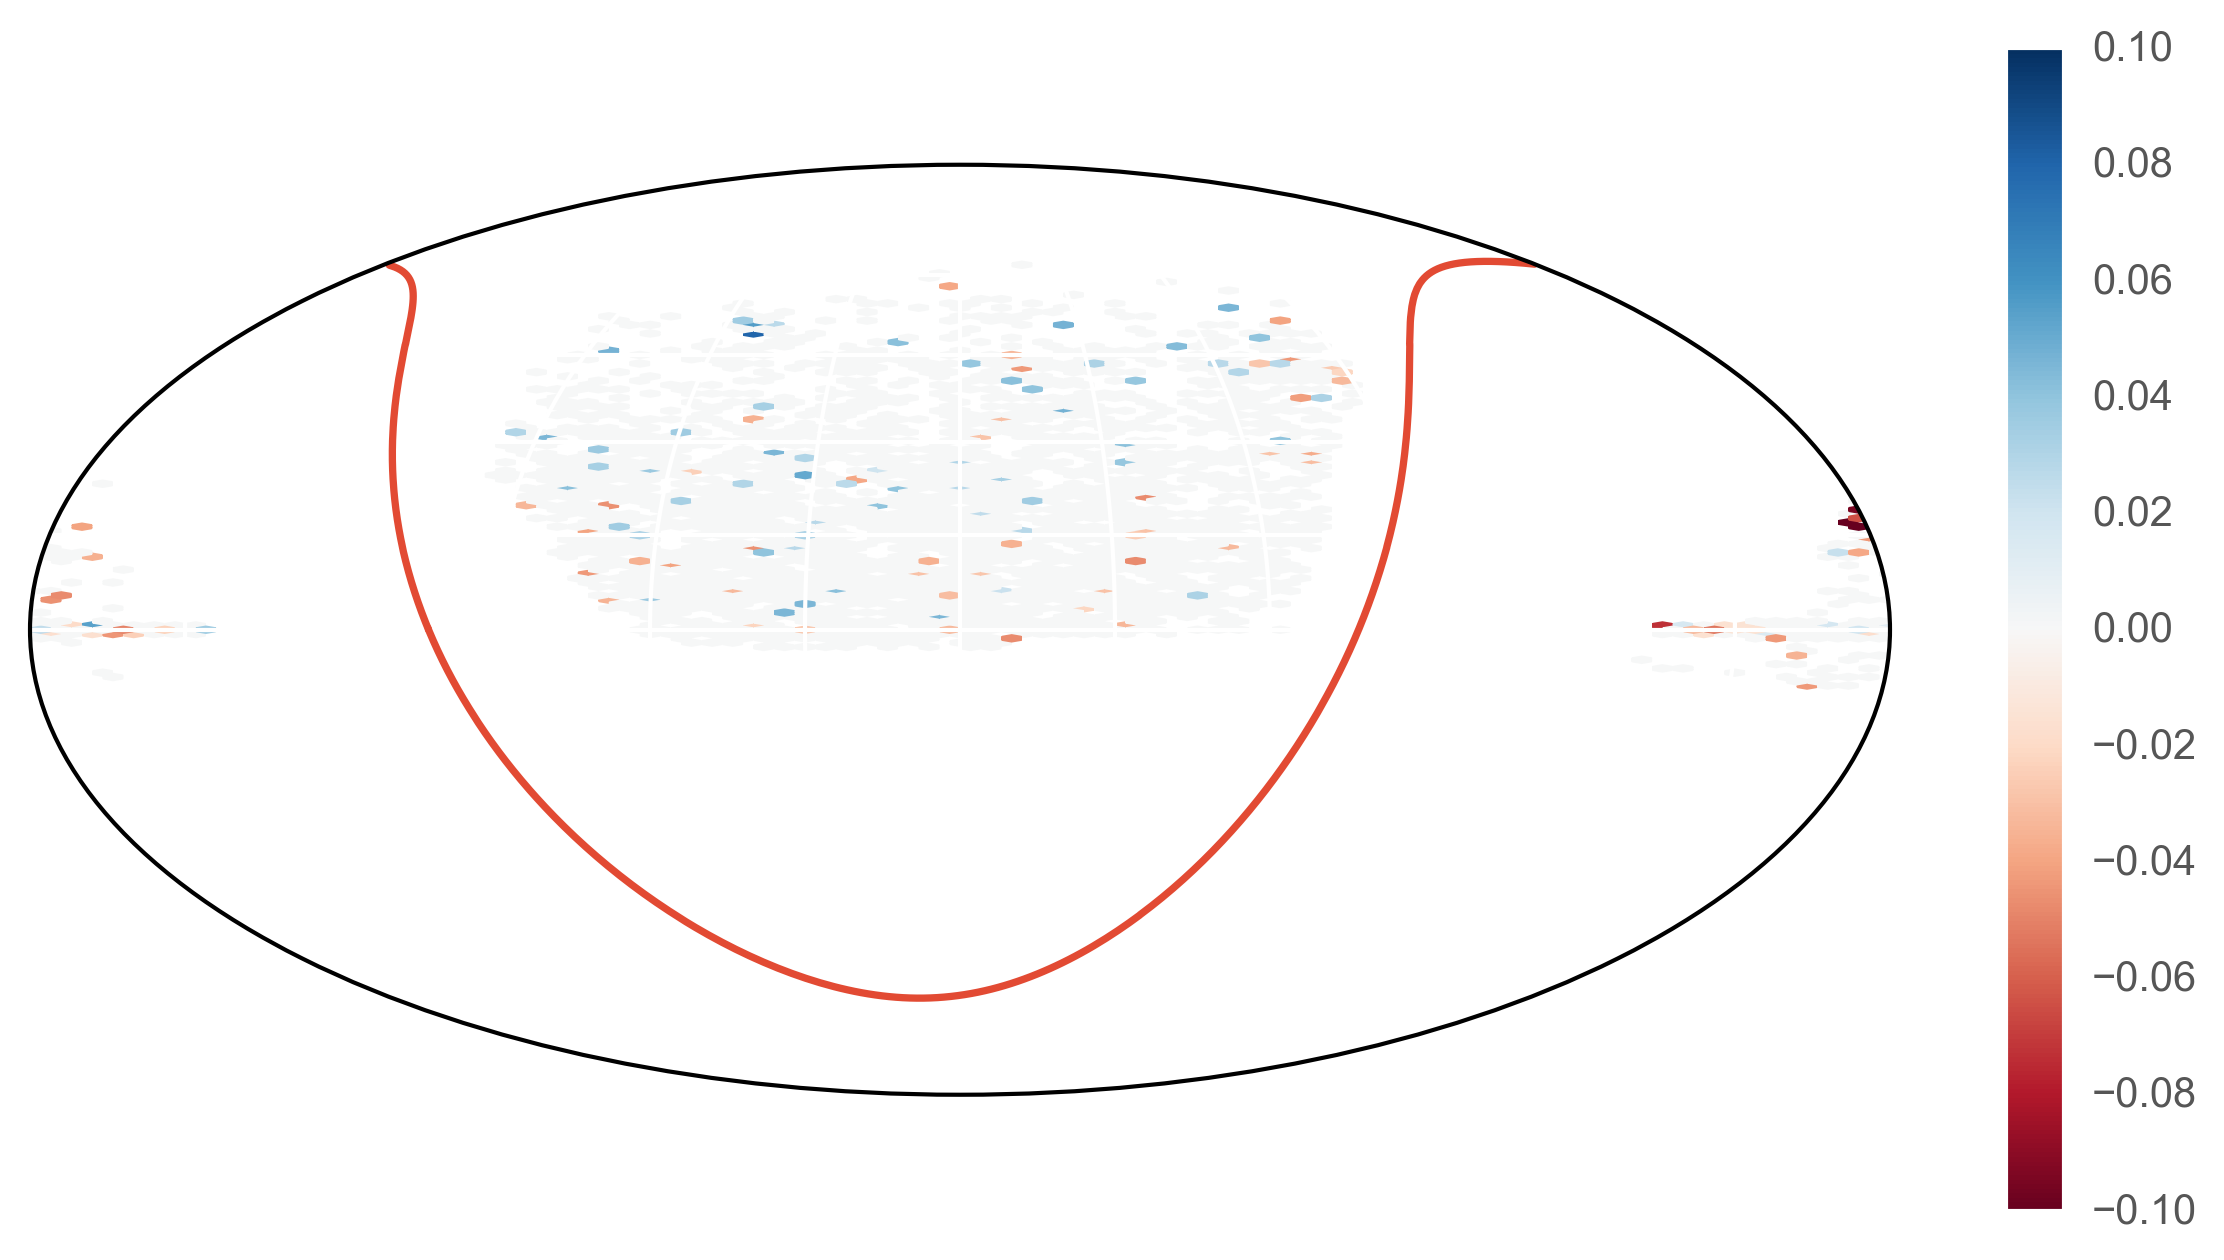
\includegraphics[width=0.75\textwidth]{figures/appendix/map_recall_w14_Galaxy}
		\caption{Recall improvement map of galaxies.}
		\label{fig:map_recall_w14_galaxies}
	\end{subfigure}\\
	\begin{subfigure}{\textwidth}
		\centering
		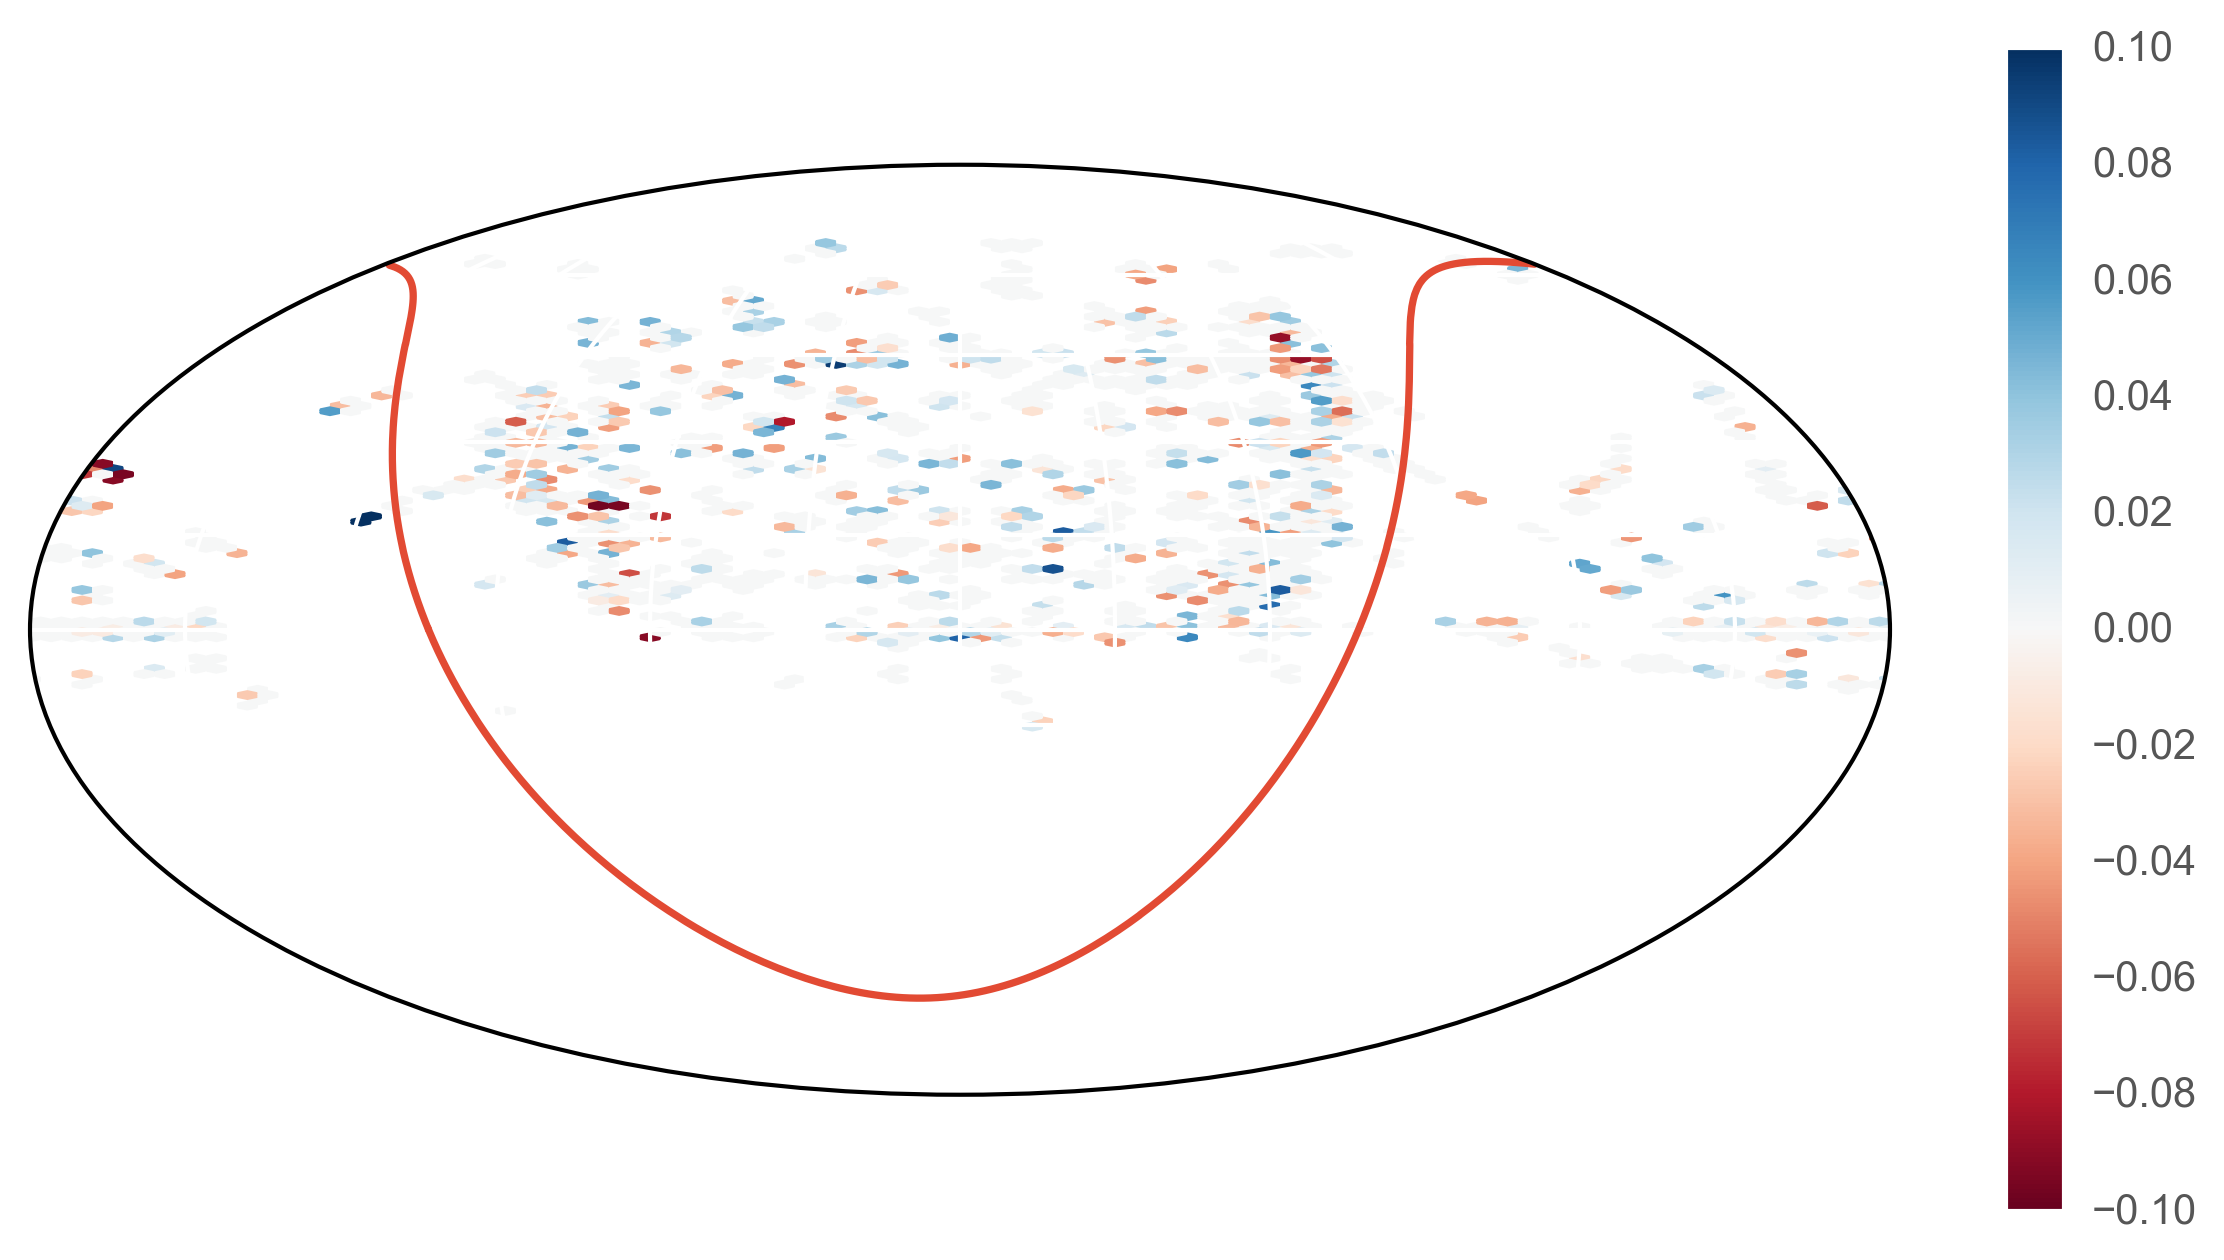
\includegraphics[width=0.75\linewidth]{figures/appendix/map_recall_w14_Star}
		\caption{Recall improvement map of stars.}
		\label{fig:map_recall_w14_stars}
	\end{subfigure}
	\begin{subfigure}{\textwidth}
		\centering
		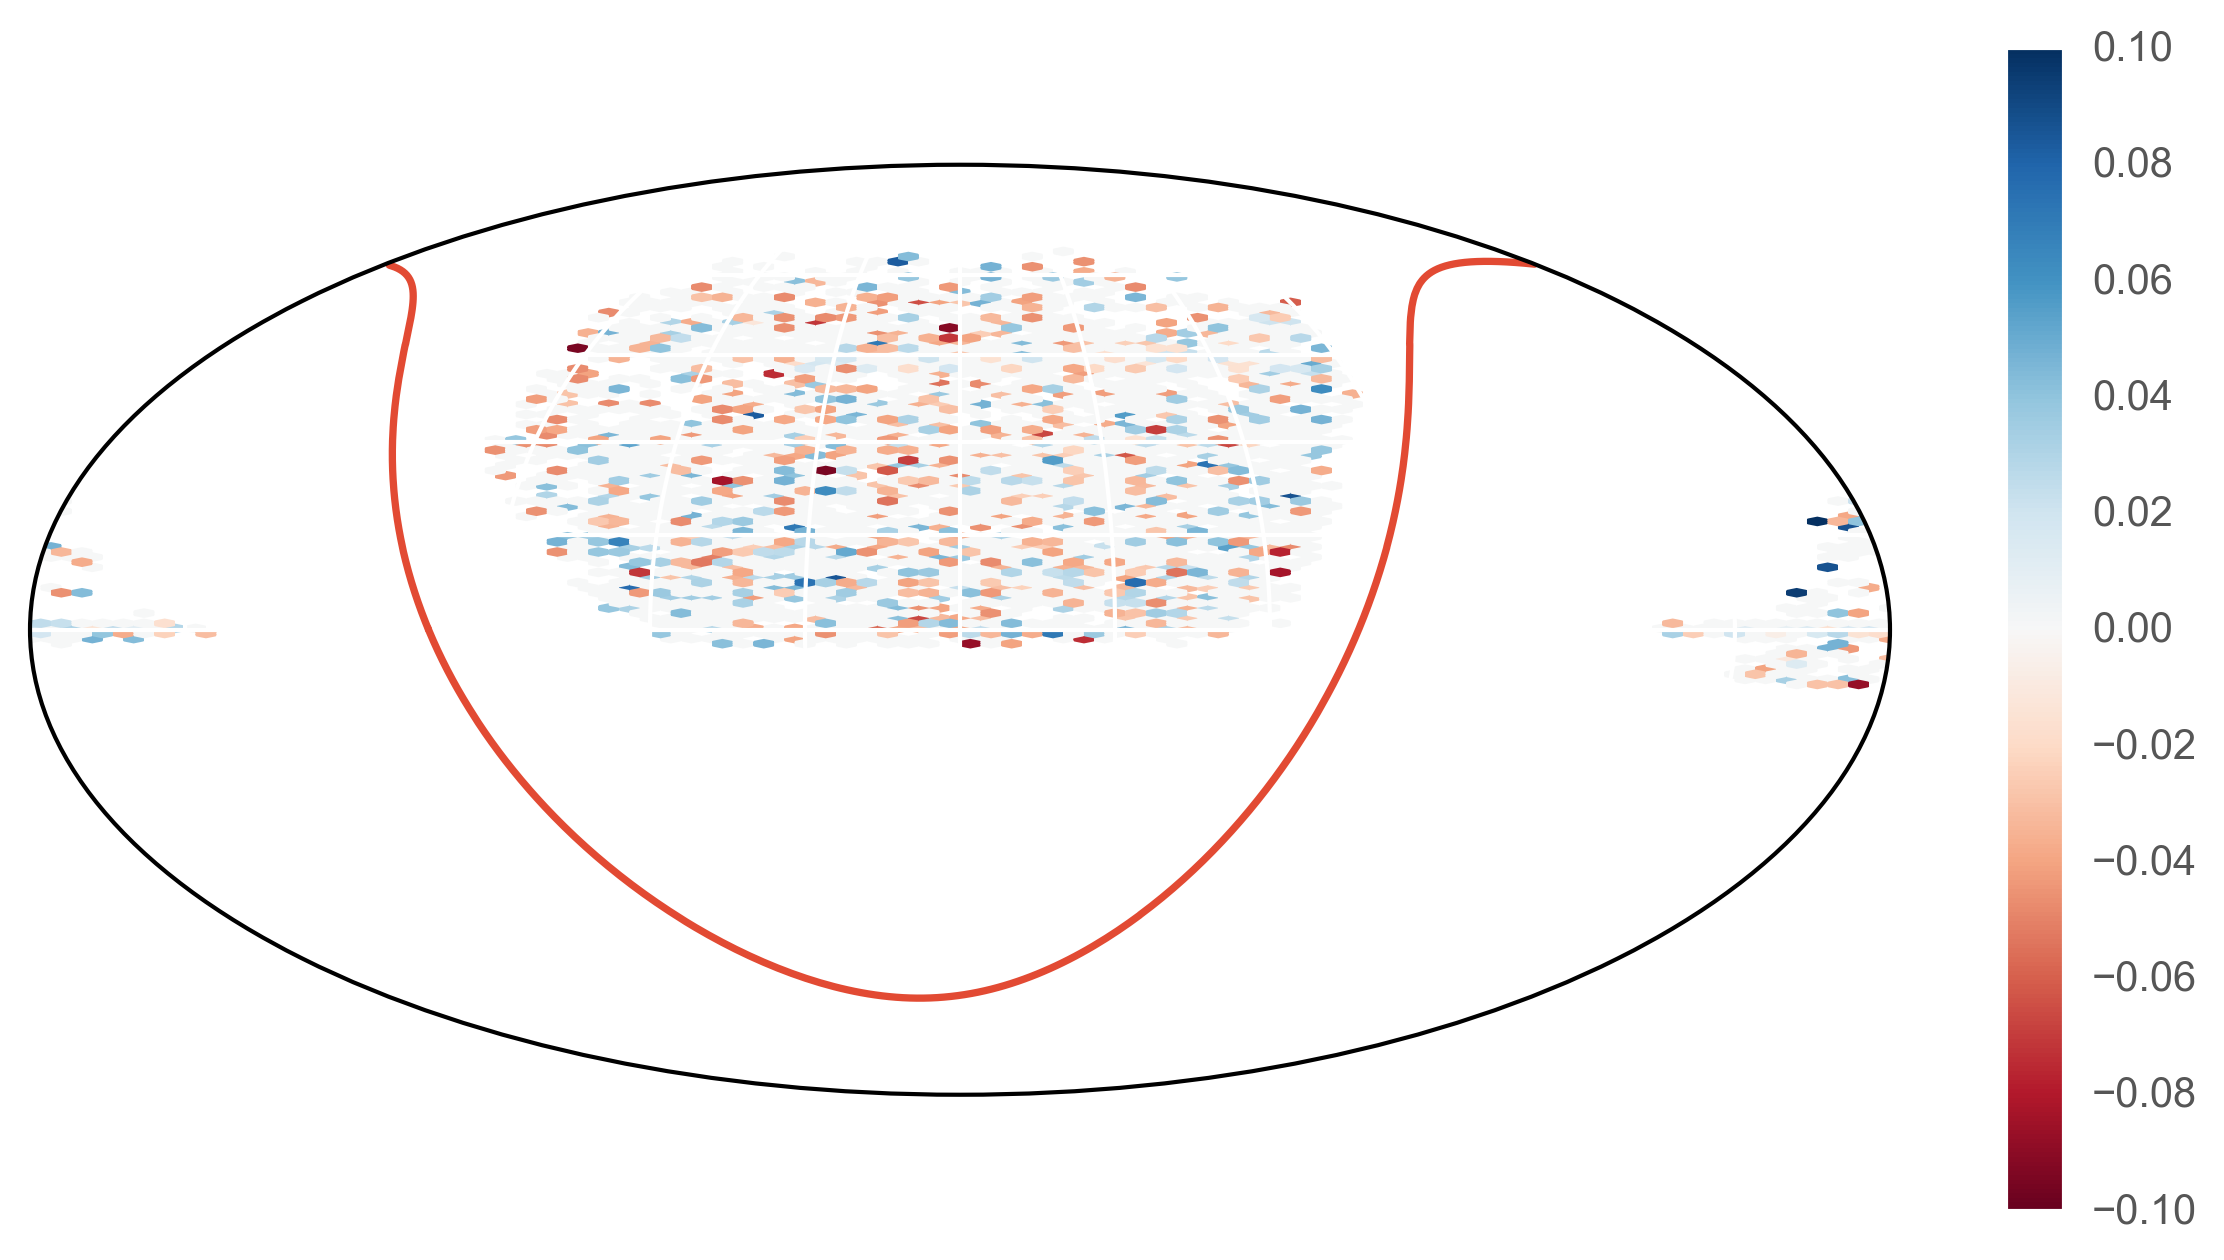
\includegraphics[width=0.75\linewidth]{figures/appendix/map_recall_w14_Quasar}
		\caption{Recall improvement map of quasars.}
		\label{fig:map_recall_w14_quasars}
	\end{subfigure}
	\caption{Recall improvement map of when the W14 correction set is applied.}
	\label{fig:map_recall_w14}
\end{figure}


\section{Variance of the Reward Function in Thompson Sampling}


\begin{figure}[p]
	\centering
	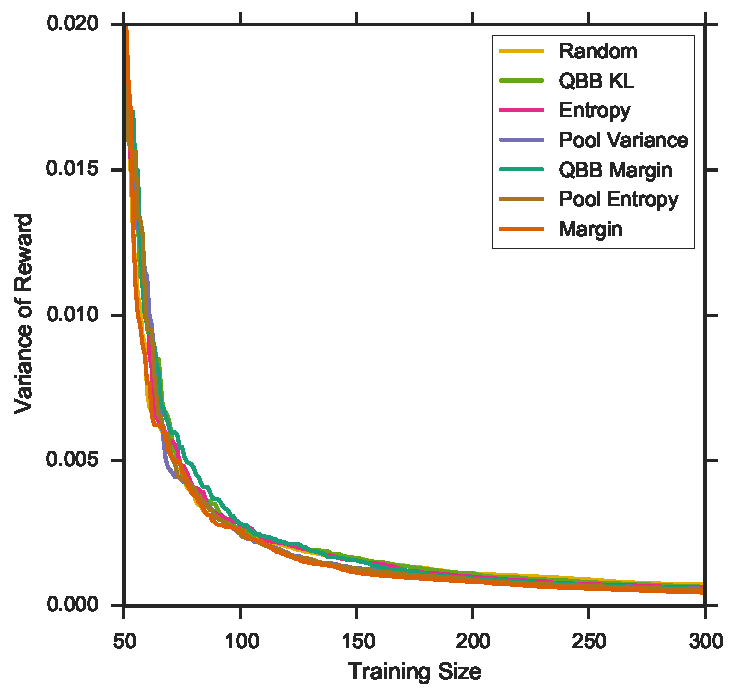
\includegraphics[width=\textwidth]{figures/5_thompson/sdss_bl_sigmas}
	\caption[Variance of the reward (SDSS, balanced, logistic)]{
		Variance of the reward (SDSS, balanced, logistic)}
	\label{fig:sdss_bl_sigmas}
\end{figure}

\begin{figure}[p]
	\centering
	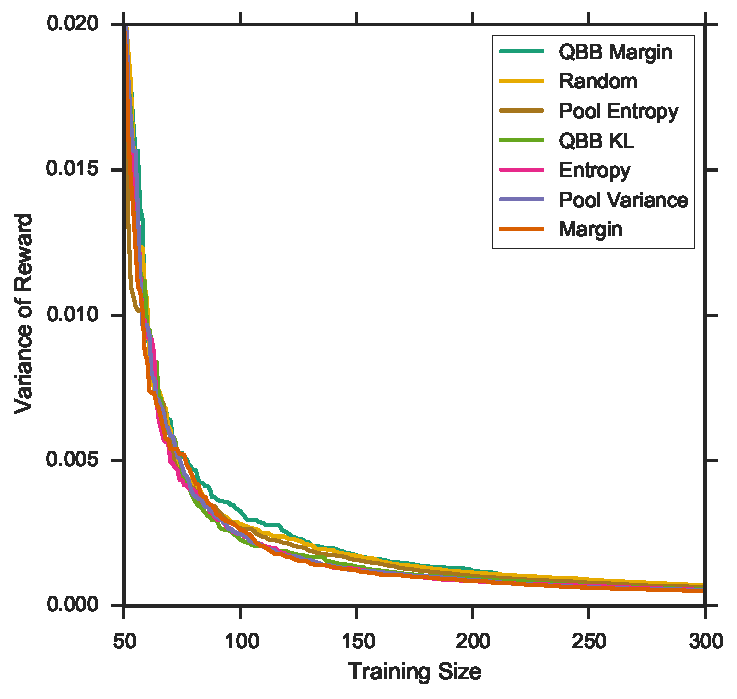
\includegraphics[width=\textwidth]{figures/5_thompson/sdss_br_sigmas}
	\caption[Variance of the reward (SDSS, balanced, SVM)]{
		Variance of the reward (SDSS, balanced, SVM)}
	\label{fig:sdss_br_sigmas}
\end{figure}

\begin{figure}[p]
	\centering
	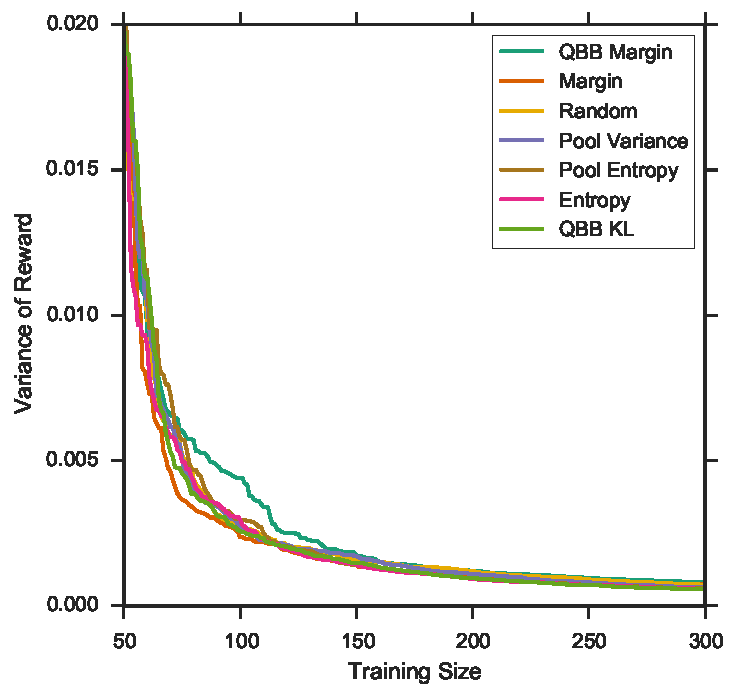
\includegraphics[width=\textwidth]{figures/5_thompson/sdss_ul_sigmas}
	\caption[Variance of the reward (SDSS, unbalanced, logistic)]{
		Variance of the reward (SDSS, unbalanced, logistic)}
	\label{fig:sdss_ul_sigmas}
\end{figure}

\begin{figure}[p]
	\centering
	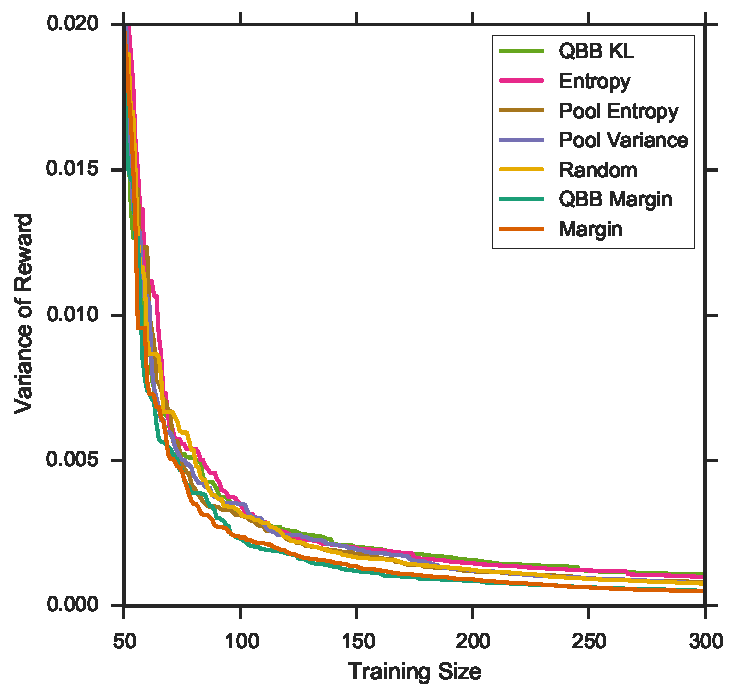
\includegraphics[width=\textwidth]{figures/5_thompson/sdss_ur_sigmas}
	\caption[Variance of the reward (SDSS, unbalanced, SVM)]{
		Variance of the reward (SDSS, unbalanced, SVM)}
	\label{fig:sdss_ur_sigmas}
\end{figure}

\begin{figure}[p]
	\centering
	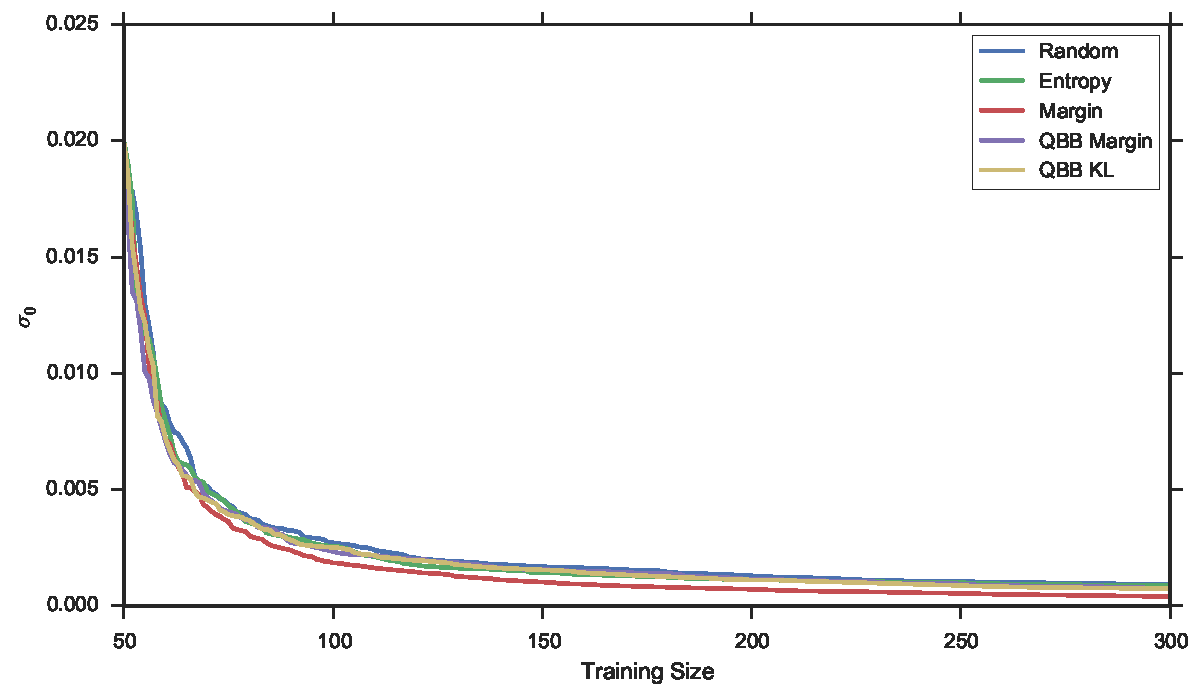
\includegraphics[width=\textwidth]{figures/5_thompson/vstatlas_bl_sigmas}
	\caption[Variance of the reward (VST ATLAS, balanced, logistic)]{
		Variance of the reward (VST ATLAS, balanced, logistic)}
	\label{fig:vstatlas_bl_sigmas}
\end{figure}

\begin{figure}[p]
	\centering
	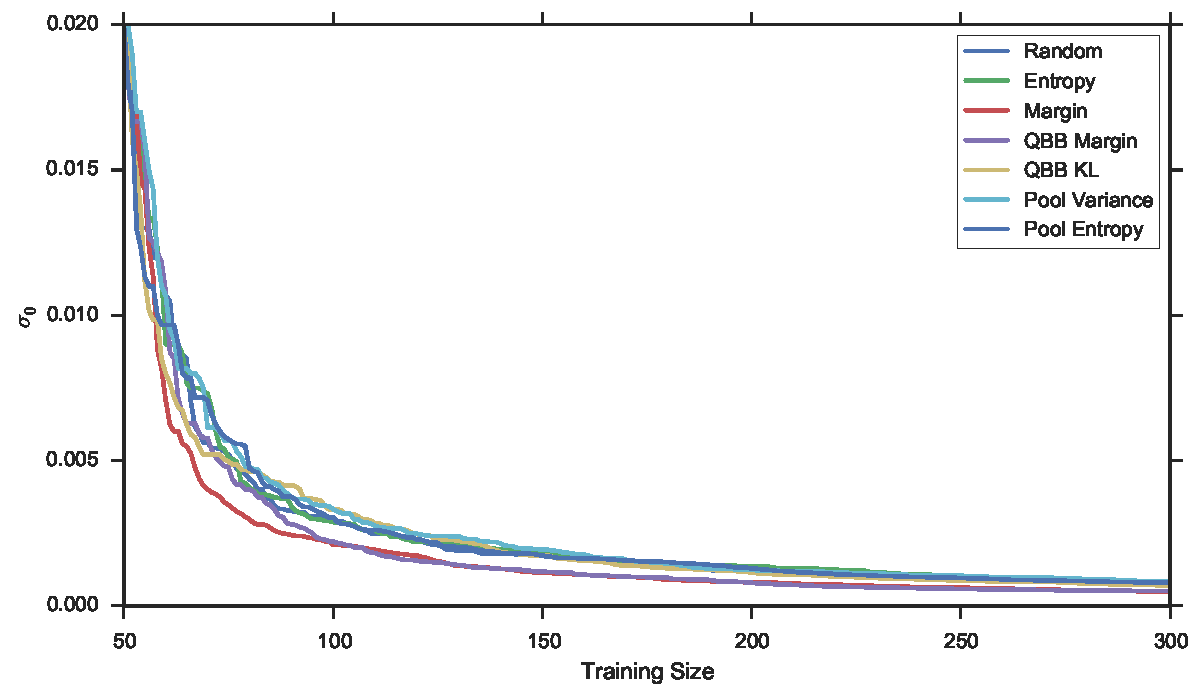
\includegraphics[width=\textwidth]{figures/5_thompson/vstatlas_br_sigmas}
	\caption[Variance of the reward (VST ATLAS, balanced, SVM)]{
		Variance of the reward (VST ATLAS, balanced, SVM)}
	\label{fig:vstatlas_br_sigmas}
\end{figure}

\begin{figure}[p]
	\centering
	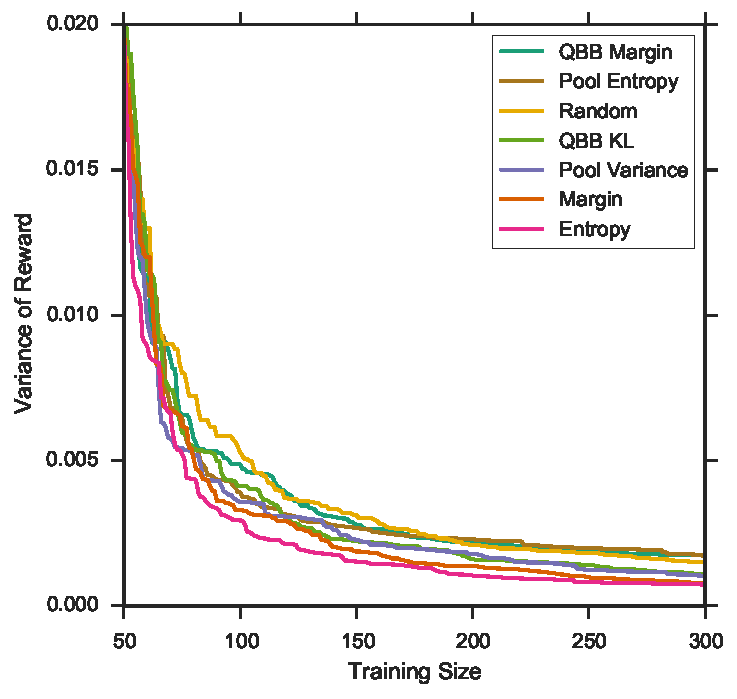
\includegraphics[width=\textwidth]{figures/5_thompson/vstatlas_ul_sigmas}
	\caption[Variance of the reward (VST ATLAS, unbalanced, logistic)]{
		Variance of the reward (VST ATLAS, unbalanced, logistic)}
	\label{fig:vstatlas_ul_sigmas}
\end{figure}

\begin{figure}[p]
	\centering
	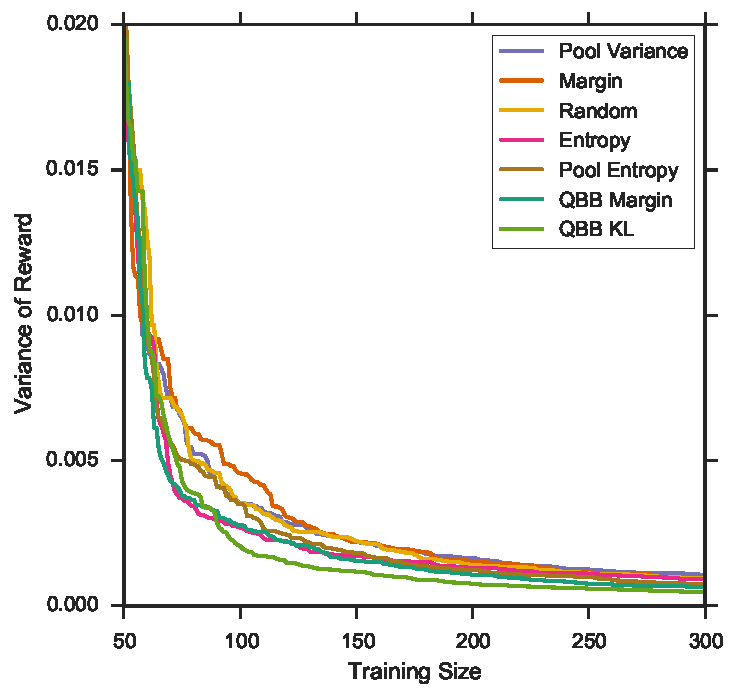
\includegraphics[width=\textwidth]{figures/5_thompson/vstatlas_ur_sigmas}
	\caption[Variance of the reward (VST ATLAS, unbalanced, SVM)]{
		Variance of the reward (VST ATLAS, unbalanced, SVM)}
	\label{fig:vstatlas_ur_sigmas}
\end{figure}


%%% Local Variables: 
%%% mode: latex
%%% TeX-master: "thesis"
%%% End: 
